\documentclass[12pt]{article}

\usepackage[utf8]{inputenc}
\usepackage{amsmath, amssymb}
\usepackage{geometry}
\usepackage{hyperref}
\usepackage{graphicx}
\usepackage{fancyhdr}
\usepackage{hyperref}
\usepackage{float}
\usepackage{subfig} % Added for subfloat functionality
% Page layout
\geometry{a4paper, margin=1in}

% Header and footer
\pagestyle{fancy}
\fancyhf{}
\fancyhead[L]{Real-Time Systems}
\fancyhead[R]{\thepage}
\setlength{\headheight}{14.49998pt} % Adjust head height
\addtolength{\topmargin}{-2.49998pt} % Compensate for the increased head height
\hypersetup{
    colorlinks,
    linkcolor=black,
    filecolor=black,      
    urlcolor=cyan,
}
\newtheorem{theorem}{Theorem}
% Title
\title{Appunti sistemi embedded \\ Scheduling in sistemi real-time}
\author{}
\date{2025}

\begin{document}

\maketitle
\tableofcontents
\newpage
\section{Introduzione}

I sistemi real time sono sistemi di computazione dove la reazione a eventi dell'ambiente deve avvenire entro precisi requisiti temporali.
Dunque la correttezza della computazione non dipende unicamente dal risultato prodotto, ma anche dal tempo in cui il risultato è prodotto.
Una reazione ritardata potrebbe essere inutile o addirittura dannosa.
Molto spesso questi sistemi vengono implementati attraverso la programmazione in assembly o con driver a basso livello per la gestione delle periferiche, manipolazione delle task 
e la priorità degli interrupt.
\\
Questo approccio presenta degli svantaggi
\begin{itemize}
    \item Programmazione tediosa
    \item Codice poco comprensibile
    \item Difficile manutenibilità
    \item Difficile verifica dei vincoli temporali
\end{itemize}
La conseguenza maggior di questo approccio è che il software costruito tramite tecniche empiriche può  essere impredicibile.\\
Se tutti i vincoli temporali critici non possono essere verificati a priori e il sistema operativo non include meccanismi specifici per maneggiare i task real-time
il sistema potrebbe apparentemente funzionare correttamente per un certo periodo di tempo, ma potrebbe fallire in situazioni particolari.
Il testing, pur essendo importante, non può essere una soluzione per ottenere la predicibilità in un sistema real-time. Questo vale perché 
il flusso di controllo dipende anche da eventi esterni dell'ambiente, che non possono essere interamente inclusi nel testing.
\section{Real time}
La correttezza del sistema non dipende solamente dal risultato logico prodotto dalla computazione ma anche dal tempo in cui il risultato è prodotto.
Il termine reale indica che la reazione del sistema a eventi esterni deve avvenire \textbf{durante} la loro evoluzione.
Di conseguenza il tempo interno al sistema deve essere misurato usando la stessa scala utilizzata per misurare il tempo dell'ambiente controllato.
Al livello di processo la principale differenza tra un task real-time e non è la presenza di una \textbf{deadline}, ovvero il tempo massimo in cui una task deve essere completata.
In un sistema critico una task che non rispetta la deadline non solo è in ritardo, è anche un errore!
In base alle conseguenze a cui porta il non rispettare la deadline le task possono essere suddivise in:
\begin{itemize}
\item \textbf{Hard} se il non rispetto della deadline porta a conseguenze catastrofiche, ad esempio il fallimento di un sistema di controllo di un aereo.
\item \textbf{Firm} se il non rispetto della deadline porta a un output inutile al sistema ma non produce conseguenze catastrofiche.
\item \textbf{Soft} se il non rispetto della deadline porta a una degradazione della qualità del servizio ma non produce conseguenze catastrofiche.
\end{itemize}
Un sistema in grado di gestire task hard real-time è detto \textbf{hard real-time system}.
Alcuni di questi sistemi sono tendenzialmente sistemi \textbf{safety critical}.
\subsection{Limiti dei sistemi real-time correnti}
Molti dei sistemi attualmente in uso sono soluzioni basate su kernel, che sono versioni modificate di sistemi operativi a time sharing.
Una conseguenza di questo è che condividono le stesse feature di base dei sistemi a time sharing, che non sono adatte a sistemi real-time.
Le caratteristiche principali sono:
\begin{itemize}
\item \textbf{Multitasking}\\
    Supporto per la programmazione concorrente offerta attraverso un insieme di chiamate a sistema per la gestione dei processi. Molte di queste primitive
    non prendono in considerazione il tempo e, peggio ancora, introducono ritardi senza limiti ai tempi di esecuzione, il che potrebbe portare le task hard a non rispettare le deadline in maniera non predicibile.
\item \textbf{Scheduling basato su priorità}\\
    Meccanismo flessibile di scheduling, dato che permette di implementare diverse strategie in base alla maniera in cui assegno le priori
    Nonostante ciò, mappare i constraint a un insieme di priorità è difficile e non sempre possibile, specialmente in un sistema dinamico.
    Il problema principale è che i kernel permettono un \textbf{numero limitato di livelli di priorità}, mentre le deadline possono variare molto di più.
    In sistemi dinamici l'arrvo di una nuova task può comportare un remappaggio dell'intero insieme di priorità.
\item \textbf{Capacità di rispondere velocemente agli interrupt}\\
    Solitamente questa feature viene ottenuta tramite la possibilità di impostare una priorità per gli interrupt, più alta rispetto alla priorità dei processi e 
    riducendo al minimo le porzioni di codice eseguite con le interruzioni disabilitate.
    \\
    Nota che questo approccio aumenta la reattività del sistema agli eventi esterni, ma introduce dei ritardi non limitati all'esecuzione dei processi.
    Infatti, un processo di un'applicazione sarà sempre interrotto da un interrupt di un driver, anche se è più importante che venga servita la periferica.
\item \textbf{Meccanismo di base per la comunicazione tra processi e sincronizzazione}\\
    Tipicamente semafori binari per la sincronizzazione e la mutua esclusione su risorse condivise.
    Però, se nessun protocollo d'accesso è utilizzato per entrare in sezioni critiche i semafori possono generare una serie di problemi, ad esempio la \textbf{priority inversion} o deadlock.
\item \textbf{Small kernel e context switch veloce}\\
    Questa feature riduce l'overhead del sistema, dunque migliora il response time medio dell'insieme di task. 
    Ciò nonostante non è sufficiente per garantire il rispetto delle deadline. D'altro canto un kernel piccolo implica limitate funzionalità, il che ha effetto sulla predicibilità del sistema.
\item \textbf{Supporto a clock real-time come reference di tempo interna}\\
    Feature essenziale di ogni kernel real-time che gestisce task hard real-time che interagiscono con l'ambiente esterno.
    Nella maggior parte dei kernel commerciali questo è l'unico meccanismo di temporizzazione disponibile.
    In molti casi non vi sono primitive per controllare esplicitamente i constraint temporali delle task, e non c'è un supporto per l'attivazione automatica delle task periodiche.
\end{itemize}
La mancanza di una qualsiasi garanzia preclude l'utilizzo di questi sistemi in casi in cui i requisiti temporali siano stringenti.
\subsection{Feature desiderabili di un sistema real-time}
La predicibilità può essere ottenuta apportando pesanti modifiche ai tipici sistemi a time sharing.
Alcune proprietà importanti sono:
\begin{itemize}
\item \textbf{Timeliness}\\
    I risultati non devono essere corretti solo nel loro valore ma anche nel dominio temporale.
    Di conseguenza il sistema operativa deve fornire degli specifici meccanismi del kernel per la gestione del tempo e 
    per la gestione dei task con constraint temporali espliciti e criticità diverse.
\item \textbf{Predicibilità}\\\
    Per raggiungere il livello di performance desiderato, il sistema deve essere analizzabile per prevedere le conseguenze di ogni decisione di scheduling.
    Nelle applicazioni safety critical tutti i requisiti temporali devono esser garantiti a priori, prima di mettere il sistema in azione.
    Se qualche vincolo non può essere garantito, il sistema deve essere in grado di informare l'utente e delle decisioni alternative devono essere prese.
\item \textbf{Efficienza}\\
    La maggior parte dei sistemi real-time sono embedded, dunque l'efficienza è un requisito fondamentale.
\item \textbf{Robustezza}\\
    Il sistema deve essere in grado di continuare a funzionare a qualsiasi condizioni di carico. La gestione dell'overload e il comportamento di adattamento sono feature essenziali per sistemi con molta varianza di carico.
\item \textbf{Tolleranza agli errori}\\
    Singoli errori hardware o software non devono portare a un fallimento del sistema.
\item \textbf{Manutenibilità}\\
    L'architettura di un sistema real-time deve essere progettata in maniera modulare per permettere di eseguire modifiche facilmente.
\end{itemize}
\section{Fonti di impredicibilità}
Un sistema dovrebbe essere in grado di prevedere l'evoluzione delle task e garantire in anticipo che tutti i vincoli temporali critici 
vengano rispettati.
L'affidabilità della garanzia dipende da un insieme di fattori, che includono anche le caratteristiche fisiche dell'hardware e 
i meccanismi/politiche del kernel.
\\
La prima componente che influisce sulla predicibilità è il processore. Le caratteristiche del processore, ad esempio il prefetch delle istruzioni, 
pipelining, cache, DMA sono fonti di \textbf{non determinismo}.
\\
Pur aumentando le performance medie del sistema, introducono fattori di non determinismo che prevengono una precisa stima dei worst-case-execution-time (WCETs).
Altre caratteristiche che influenzano la predicibilità sono le caratteristiche interne del kernel, come l'algoritmo di scheduling, i meccanismi di sincronizzazione, 
i tipi di semafori, le politiche di gestione della memoria e le politiche di gestione degli interrupt.
\subsection{DMA}
Uno dei modi più comuni per implementarlo è tramite cycle stealing, il DMA controller prende il controllo del bus per un ciclo di clock 
e poi lo rilascia al processore.
Durante l'operazione di DMA il trasferimento e l'esecuzione del codice sul processore avvengo in parallelo.
SE la CPU e il DMA controller richiedono un ciclo di memoria allo stesso tempo, il bus viene assegnato al DMA controller e la CPU
aspetta finché il DMA non ha finito.
In questo modo non è possibile prevedere il tempo di esecuzione di un task, dato che il tempo di esecuzione dipende da quante volte il DMA controller ha bisogno del bus.
\\
Una possibile soluzione al problema è il time slicing, dove un ciclo di memoria è diviso in due slot di tempo adiacenti, uno per il DMA e uno per la CPU.
Questa soluzione è più costosa ma più prevedibile di cycle stealing, dato che il response time di una task non è influenzato dal DMA.
\subsection{Cache}
Nei sistemi real-time la cache è una fonte di non determinismo, dato che il tempo di accesso alla memoria dipende dalla presenza o meno del dato in cache.
Quando avviene un cache miss il tempo di accesso alla memoria è molto più lungo, e questo non è prevedibile.
Quando si effettua una scrittura in memoria l'utilizzo della cache risulta costoso perché il tempo di accesso alla memoria è più lungo, dato che deve essere garantita la consistenza.
\subsection{Interrupts}
Un grosso problema per la predicibilità è la gestione degli interrupt provenienti dalle periferiche I/O.
Se non gestite correttamente possono introdurre ritardi non limitati durante l'esecuzione di processi.\\
In quasi tutti i sistemi operativi la gestione di un interrupt prevede l'esecuzione di una service routine dedicata per la gestione del device.
Il vantaggio di questo metodo è che tutti i dettagli hardware sono contenuti nel driver.\\
In molti OS gli interrupt vengono serviti usando un sistema a priorità fissa, tramite i quali ogni driver viene schedulato in base a una priorità statica, questa priorità è più alta rispetto a quella di qualsiasi processo.
In generale è molto difficile prevedere a priori il numero di interrupt che un task può ricevere, dunque il delay è impredicibile.
\\
Per ridurre l'interferenza dei driver sui task ed effettuare operazioni di I/O le periferiche devono essere gestiste differentemente
\subsubsection{Approccio A}
La soluzione più radicale è disattivare tutti gli interrupt esterni, a eccezione di quelli generati dal timer.
Tutte le periferiche vanno gestiste dall'applicazione (controllo di programma), i quali hanno accesso ai registri delle periferiche.
Dato che non ci sono più interrupt, il trasferimento deve essere effettuato tramite polling.
L'accesso diretto alle periferiche consente alta flessibilità al livello di programma ed elimina i delay introdotti dai driver.
Dunque il tempo necessario per un trasferimento può essere calcolato a priori.
Un altro vantaggio è che il kernel non va modificato quando una nuova periferica viene aggiunta o ne viene rimossa una.
\\
Lo svantaggio principale è che risulta poco efficiente dato la busy wait necessaria per il polling.
Un grosso problema è che le applicazioni richiedono la conoscenza completa dei dettagli a basso livello delle periferiche che devono gestire.
Questo può essere gestito incapsulando le routine che dipendono dai device in una libreria.
\subsubsection{Approccio B}
Come nella soluzione precedente tutti gli interrupt esterni sono disabilitati,
tranne quelli dei timer.\\
In questa soluzione le periferiche non vengono gestite direttamente dall'applicazione, ma a turno da routine dedicate del kernel 
periodicamente attivate dal timer.
Questo approccio elimina i ritardi causati dai driver e confina le operazioni di I/O a una o più routine periodiche del kernel.
In alcuni sistemi i device I/O vengono suddivisi in due gruppi in base alla loro velocità, quelli più veloci vengono gestiti da task 
periodici con frequenza maggiore.
\\
Il vantaggio di questo metodo è che tutti i dettagli hardware sono incapsulati nel kernel, dunque l'applicazione non ha bisogno di 
conoscere i dettagli a basso livello delle periferiche.
Dato che gli interrupt sono disabilitati il maggior problema è dato dalla busy wait delle procedure di gestione dell'I/O del kernel.
Questo metodo introduce un overhead maggiore rispetto all'approccio A, richiede modifiche al kernel quando una periferica viene aggiunta o rimossa.
\subsubsection{Approccio C}
Lasciare gli interrupt abilitati e ridurre al minimo possibile i driver per le periferiche.
L'unico scopo dei driver è quello di attivare una task che gestisce il device. Una volta attivato il task di gestione del device 
viene eseguito sotto diretto controllo del sistema operativo
ed è schedulato come un task normale.
In questo modo la priorità che può essere assegnata al task di gestione del device è completamente indipendente dalle altre priorità 
e può essere impostata in base ai requisiti del programma.
\begin{figure*}[h]
\centering
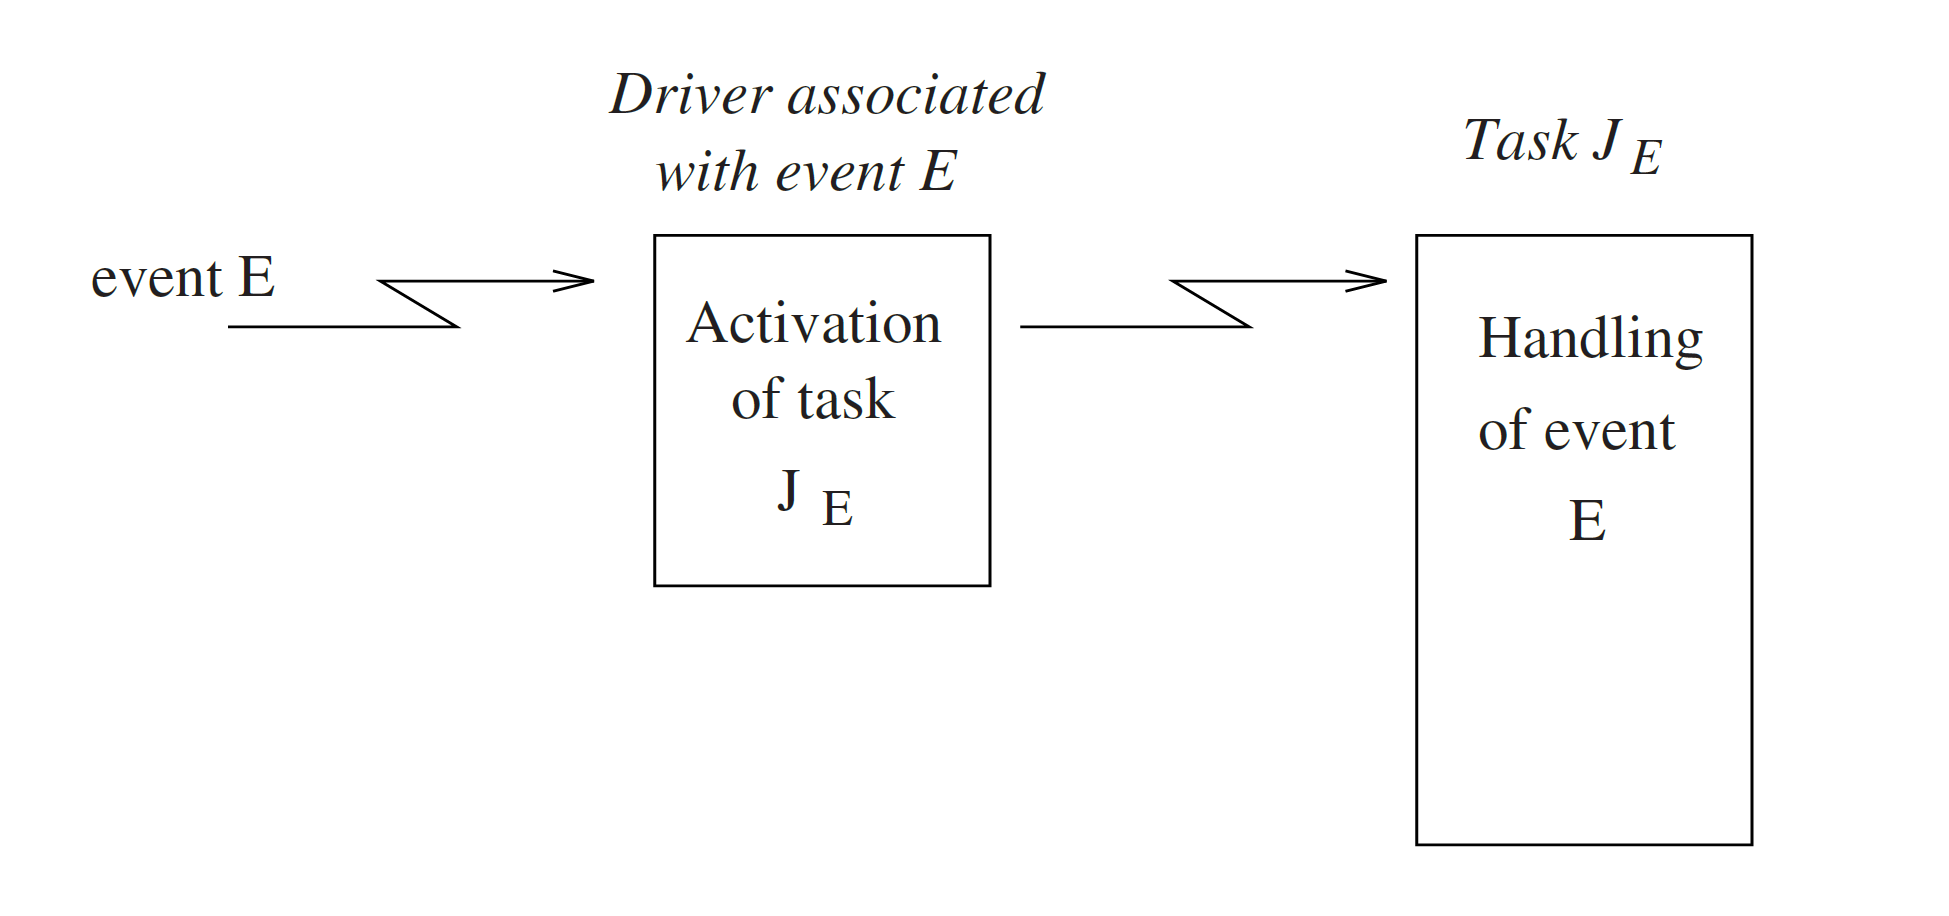
\includegraphics[height=150px]{pictures/approccioC.png}
\caption{Attivazione task per la gestione del device}
\end{figure*}
\\
Il vantaggio principale di questo metodo è che il busy wait viene eliminato e il tempo di esecuzione del driver di gestione del device è 
molto ridotto, di conseguenza il tempo di esecuzione del task è più prevedibile.
Nella maggior parte delle applicazioni pratiche il piccolo overhead portato da questo tipo di driver viene ignorato.

\subsection{Semafori}
L'usuale meccanismo dei semafori utilizzato nei sistemi operativi tradizionali non è adatto per i sistemi real-time per via del fenomeno dell'\href{https://en.wikipedia.org/wiki/Priority_inversion}{inversione di priorità}.
L'inversione di priorità deve essere evitato a tutti i costi in un sistema real-time, dato che introduce non determinismo sull'esecuzione di task critiche.
Per quanto riguarda il problema della mutua esclusione l'inversione di priorità può essere evitata usando protocolli specifici che devono essere usati ogni 
volta che si effettua un accesso alla sezione critica.
L'implementazione di questo tipo di protocollo potrebbe richiedere estensive modifiche al kernel, che non comprendono solo le primitive $wait$ e $signal$, ma anche strutture dati e meccanismi di task management.
\subsection{Gestione della memoria}
Come gli altri aspetti del kernel, la gestione della memoria deve essere progettata per evitare il non determinismo.
Ad esempio sistemi di paging on-demand non sono adatti a sistemi con rigidi vincoli temporali a causa dei lunghi e imprevedibili ritardi causati dalle page fault e page replacement.
LE soluzioni tipiche adottate nei sistemi real-time prevedono regole di segmentazione della memoria con uno schema fisso. Il partizionamento statico è particolarmente efficace quando i programmi richiedono
una quantità di memoria simile tra loro.
In generale gli schemi di allocazione statici aumentato la predicibilità del sistema, ma diminuiscono la flessibilità in sistemi dinamici, dunque la scelta progettuale va fatta bilanciando le due caratteristiche.
\subsection{Linguaggi di programmazione}
Con l'aumentare della complessità dei sistemi real-time aumenta anche la necessità di utilizzare astrazioni offerte dai linguaggi.
\\
Purtroppo i linguaggi attualmente a disposizioni non sono abbastanza espressivi da permettere di esprimere certi comportamenti temporali, dunque non sono adatti per la programmazione di sistemi real-time.
L'esistenza di costrutti che modificano il flusso di controllo del programma in maniera non deterministica, come gli $if$, rende impossibile la stima affidabile dei WCETs in attività concorrenti.
Un'altra fonte di impredicibilità è data dalla ricorsione, l'analizzatore di scheduling non è in grado di prevedere il numero di chiamate ricorsive e il tempo di esecuzione.

\section{Concetti di base di scheduling}
\subsection{Introduzione}
Un \textbf{processo} è una computazione eseguita dalla CPU in maniera sequenziale, d'ora in poi useremo il termine processo come sinonimo di \textit{task} o \textit{thread}.
\\
In realtà un processo è una entità più complessa composta da vari task (o thread)
che condividono lo stesso spazio di indirizzamento e le stesse risorse.
Una \textbf{politica di scheduling} è un criterio secondo il quale la CPU viene assegnata ai vari task che si sovrappongono.
L'insieme di politiche che in ogni istante di tempo determinano l'ordine con il quale i task vengono eseguiti è detto \textbf{algoritmo di scheduling}.\\
L'operazione specifica di assegnare la CPU a un task selezionato dall'algoritmo di scheduling è detta \textbf{dispatching}.
Quando un processo può essere potenzialmente eseguito dalla CPU, possiamo avere due casi: 
\begin{itemize}
    \item Il processo è in \textbf{running} perché è già stato selezionato dall'algoritmo di scheduling e la CPU è stata assegnata a lui.
    \item Il processo è in \textbf{ready} e aspetta di essere selezionato dall'algoritmo di scheduling.
\end{itemize}
In entrambi i casi il processo viene detto un task \textbf{attivo}. Tutti i processi in wait vengono tenuti in una \textbf{ready queue}. I vari sistemi operativi possono utilizzare anche più code dipendentemente dal tipo di task.
\begin{figure}
\centering
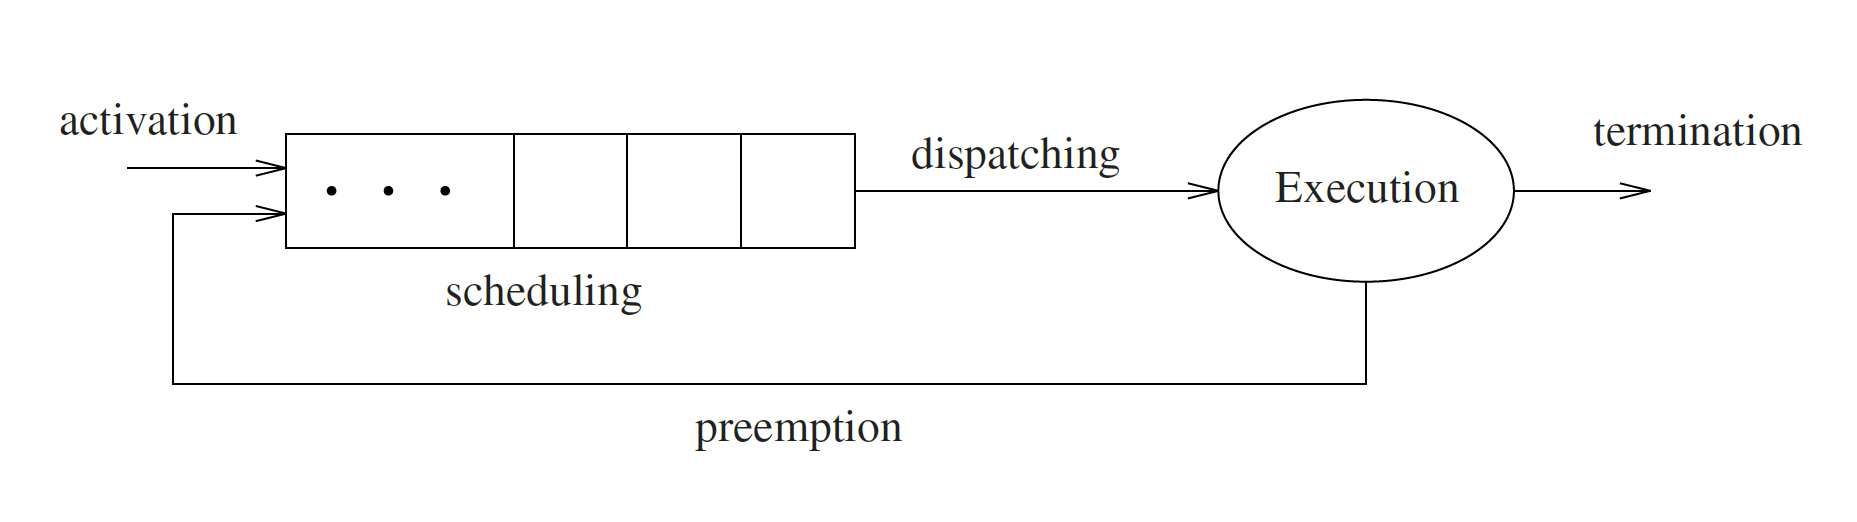
\includegraphics[width=\textwidth]{pictures/cicloEsecuzione.png}
\caption{Coda di task in ready che aspettano di essere eseguiti}
\end{figure}
In molti sistemi dove è concessa l'attivazione dinamica dei task, questi possono essere interrotti in qualsiasi momento, così che quando un task più importante entra nel sistema esso possa essere eseguito immediatamente senza aspettare nella ready queue.
L'operazione di interrompere il task in esecuzione e reinserirlo nella ready queue è detta \textbf{preemption}.\\
Nei sistemi real-time la preemption è importante per 3 motivi:
\begin{itemize}
    \item I task che gestiscono le eccezioni potrebbero aver bisogno di fare preemption di task in esecuzione per garantire che le eccezioni siano gestite in tempo.
    \item Quando i task hanno livelli di priorità diversi, i task critici possono essere eseguiti immediatamente.
    \item Tipicamente lo scheduling con preemption permette maggiore efficienza, nel senso che permette l'esecuzione di task real time con una percentuale di utilizzo di CPU maggiore.
\end{itemize}
D'altro canto la preemption distrugge la località dei programmi e introduce overhead, di conseguenza limitare la preemption in un sistema real-time può essere benefico.
\\
Uno schedule è detto \textbf{feasible} se tutti i task possono essere eseguiti rispettando l'insieme di vincoli a essi posti.
Un insieme di task è detto \textbf{schedulabile} se esiste uno schedule che rispetta i vincoli di tutti i task.
\subsection{Tipi di vincoli di scheduling}
Tipicamente i vincoli applicabili a task real time rientrano in tre classi:
\begin{itemize}
    \item Vincoli temporali
    \item Vincoli di precedenza
    \item Vincoli di mutua esclusione su risorse condivise
\end{itemize}
\subsubsection{Vincoli temporali}
I sistemi realtime sono caratterizzati da attività computazionali con stringenti vincoli temporali che devono essere rispettati per ottenere il comportamento desiderato.
Un requisito tipico è che un task deve essere completato entro un certo tempo, detto \textbf{deadline}.\\
Se la deadline è rappresentata in rispetto a quando il task è stato attivato, essa è detta \textbf{relative deadline}, altrimenti è detta \textbf{absolute deadline}.\\
In base alle conseguenze a cui porta il non rispetto della deadline le task possono essere suddivise in:
\begin{itemize}
    \item \textbf{Hard} se il non rispetto della deadline porta a conseguenze catastrofiche, ad esempio il fallimento di un sistema di controllo di un aereo.
    \item \textbf{Firm} se il non rispetto della deadline porta a un output inutile al sistema ma non produce conseguenze catastrofiche.
    \item \textbf{Soft} se il non rispetto della deadline porta a una degradazione della qualità del servizio ma non produce conseguenze catastrofiche.
\end{itemize}
\begin{figure}[h]
    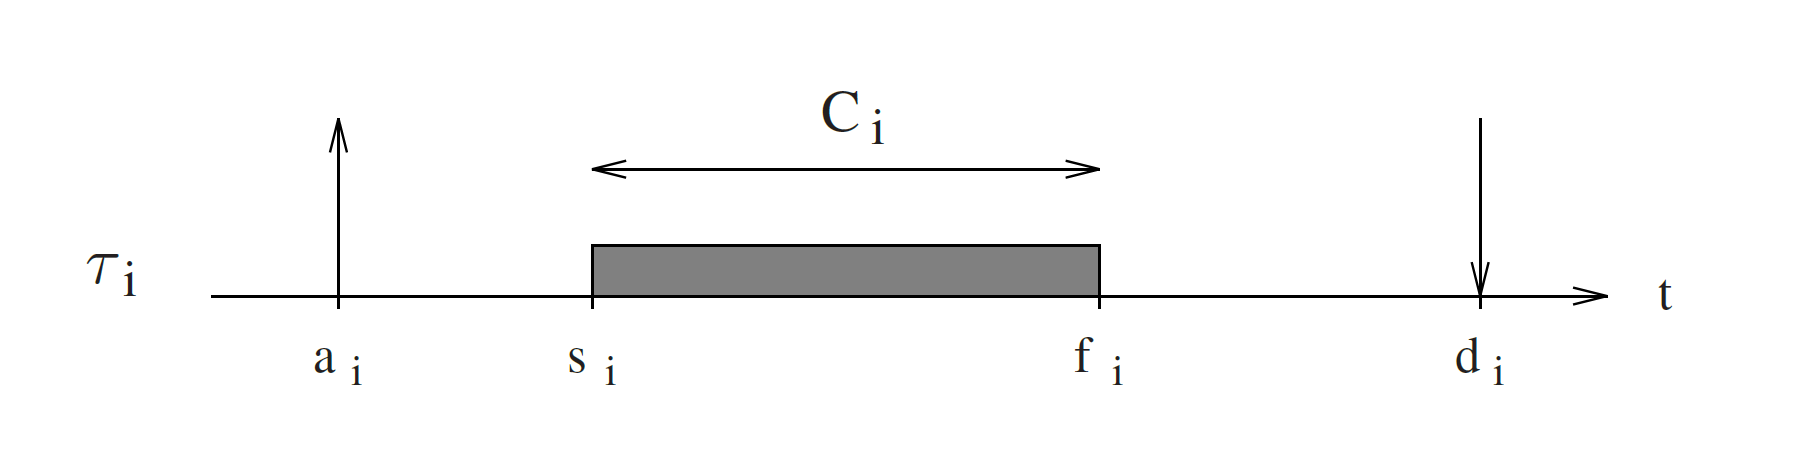
\includegraphics[width=\textwidth]{pictures/parametriTask.png}
    \caption{Parametri di un task}
\end{figure}
In generale un task realtime $\tau_i$ è caratterizzato da:
\begin{itemize}
    \item \textbf{Tempo di arrivo} $a_i$, il momento in cui il task è pronto per essere eseguito, anche detto \textbf{release time} o \textbf{request time} e indicato da $r_i$.
    \item \textbf{Tempo di computazione} $c_i$, il tempo necessario per completare il task\\ \underbar{\textbf{senza interruzioni}}, l'upperbound è il WCET.
    \item \textbf{Deadline assoluta} $d_i$, il tempo entro il quale il task deve essere completato.
    \item \textbf{Deadline relativa} $D_i$, il tempo entro il quale il task deve essere completato rispetto al suo tempo di arrivo, $D_i=d_i-r_i$.
    \item \textbf{Tempo di inizio} $s_i$, il tempo in cui il task inizia a essere eseguito.
    \item \textbf{Tempo di completamento} $f_i$, il tempo in cui il task termina la sua esecuzione.
    \item \textbf{Tempo di risposta} $T_i$, il tempo di ritardo del task, ovvero $T_i=f_i-r_i$.
    \item \textbf{Criticità}, già discusso: hard, firm o soft.
    \item \textbf{Lateness} $L_i$, il tempo di ritardo del task rispetto alla deadline, ovvero $L_i=f_i-d_i$, in generale vogliamo che sia negativa, ovvero i task devono essere eseguiti entro le deadline.
    \item \textbf{Tempo di slack} $X_i=d_i-a_i-c_i$, il tempo massimo per cui l'attivazione di un task può essere ritardata senza violare la deadline.
\end{itemize}
Un'altra caratteristica temporale che riguarda la regolarità dell'attivazione di un task.
Un task è detto \textbf{periodico} se consiste di una infinita sequenza di attività identiche, chiamate \textbf{job}, che si attivano a intervalli regolari.
Per chiarezza di notazione notiamo i task periodici con $\tau_i$ e quelli aperiodici con $J_i$. Il generico k-esimo job di un task periodico $\tau_i$ è denotato con $\tau_{i,k}$.
Il tempo di attivazione della prima istanza di un task periodico ($\tau_{i,1}$) è detto \textbf{fase}, denotato con $\phi_i$.
Il periodo di attivazione di un task periodico è denotato con $T_i$, che è il tempo tra due attivazioni consecutive.
I task \textbf{aperiodici} sono caratterizzati da un tempo di attivazione non regolare, un task \textbf{sporadico} è un task aperiodico che ha un tempo di attivazione massimo, ovvero il tempo minimo tra due attivazioni consecutive.\\
\subsubsection{Vincoli di precedenza}
In alcune applicazioni le attività non possono essere eseguite in ordine arbitrario, ma devono rispettare un ordine di precedenza stabilito durante la progettazione.
Tali precedenze tendenzialmente vengono rappresentate tramite un grafo diretto aciclico (DAG), dove i nodi rappresentano le attività e gli archi rappresentano le precedenze.
Un DAG definisce un relazione di ordine parziale tra le attività, che può essere usata per determinare un ordine di esecuzione.
\begin{figure}[H]
    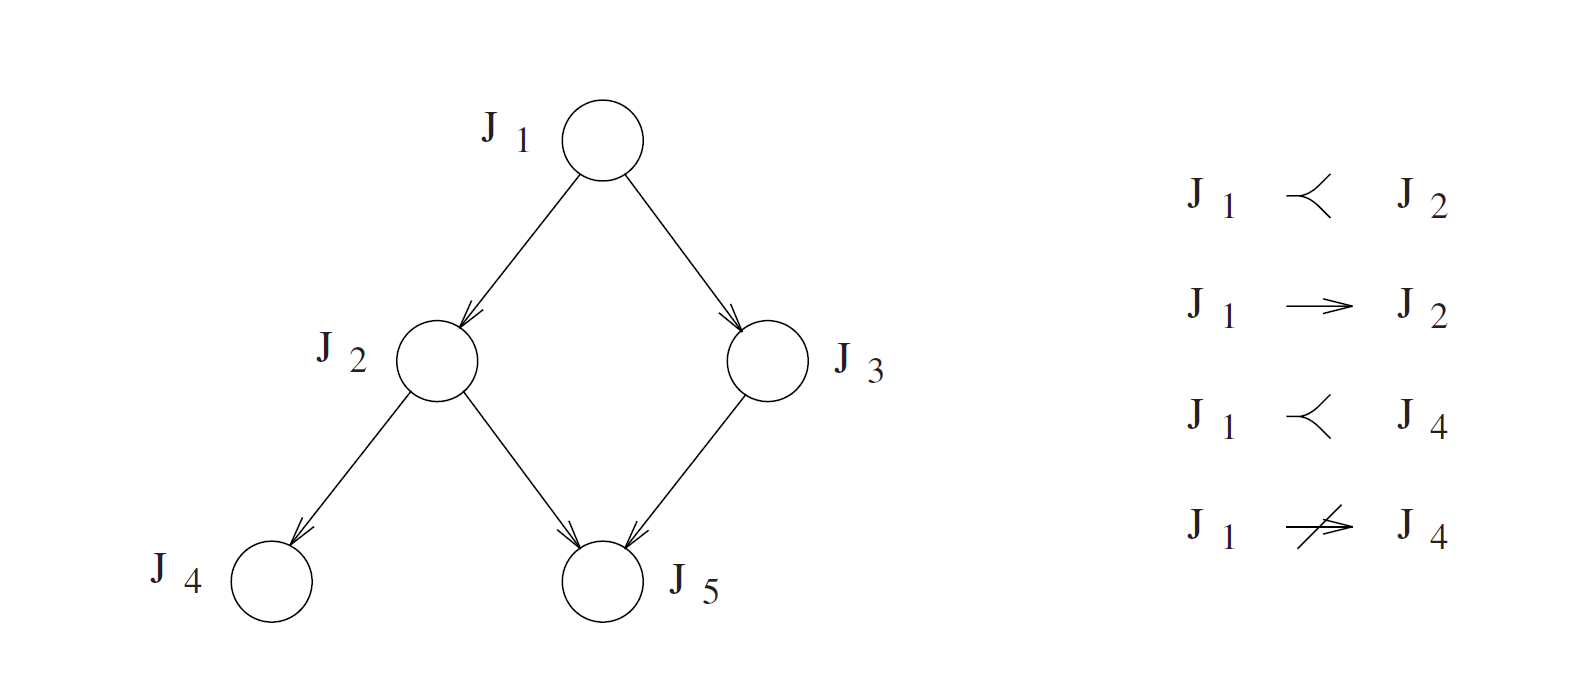
\includegraphics[width=\textwidth]{pictures/precedenzaTask.png}
    \caption{Relazione di precedenza tra 5 task}
\end{figure}
\noindent La notazione $J_a \prec J_b$ indica che il task $J_a$ è un predecessore di $J_b$, ovvero il grafo contiene un cammino orientato da $J_a$ a $J_b$.
\\
La notazione $J_a \rightarrow J_b$ indica che $J_a$ è un predecessore diretto di $J_b$, ovvero il grafo contiene un arco diretto da $J_a$ a $J_b$.
\\
I task senza predecessori vengono detti \textbf{task iniziali}, mentre quelli senza successori vengono detti \textbf{task finali}.
\subsubsection{Vincoli di mutua esclusione}
Dal punto di vista di un processo, una risorsa è una struttura software che può essere utilizzata dal processo per avanzare la sua esecuzione.
Una risorsa è detta \textit{privata} se è dedicata a un processo, altrimenti se può essere utilizzata da più processi è detta \textbf{condivisa}.
Per mantenere la correttezza del dato, molte risorse condivise non permettono l'accesso simultaneo da parte di task concorrenti, dunque richiedono la \textbf{mutua esclusione}.
La parte di codice che accede alla risorsa condivisa in mutua esclusione è detta \textbf{sezione critica}.
\begin{figure}[H]
    \centering
    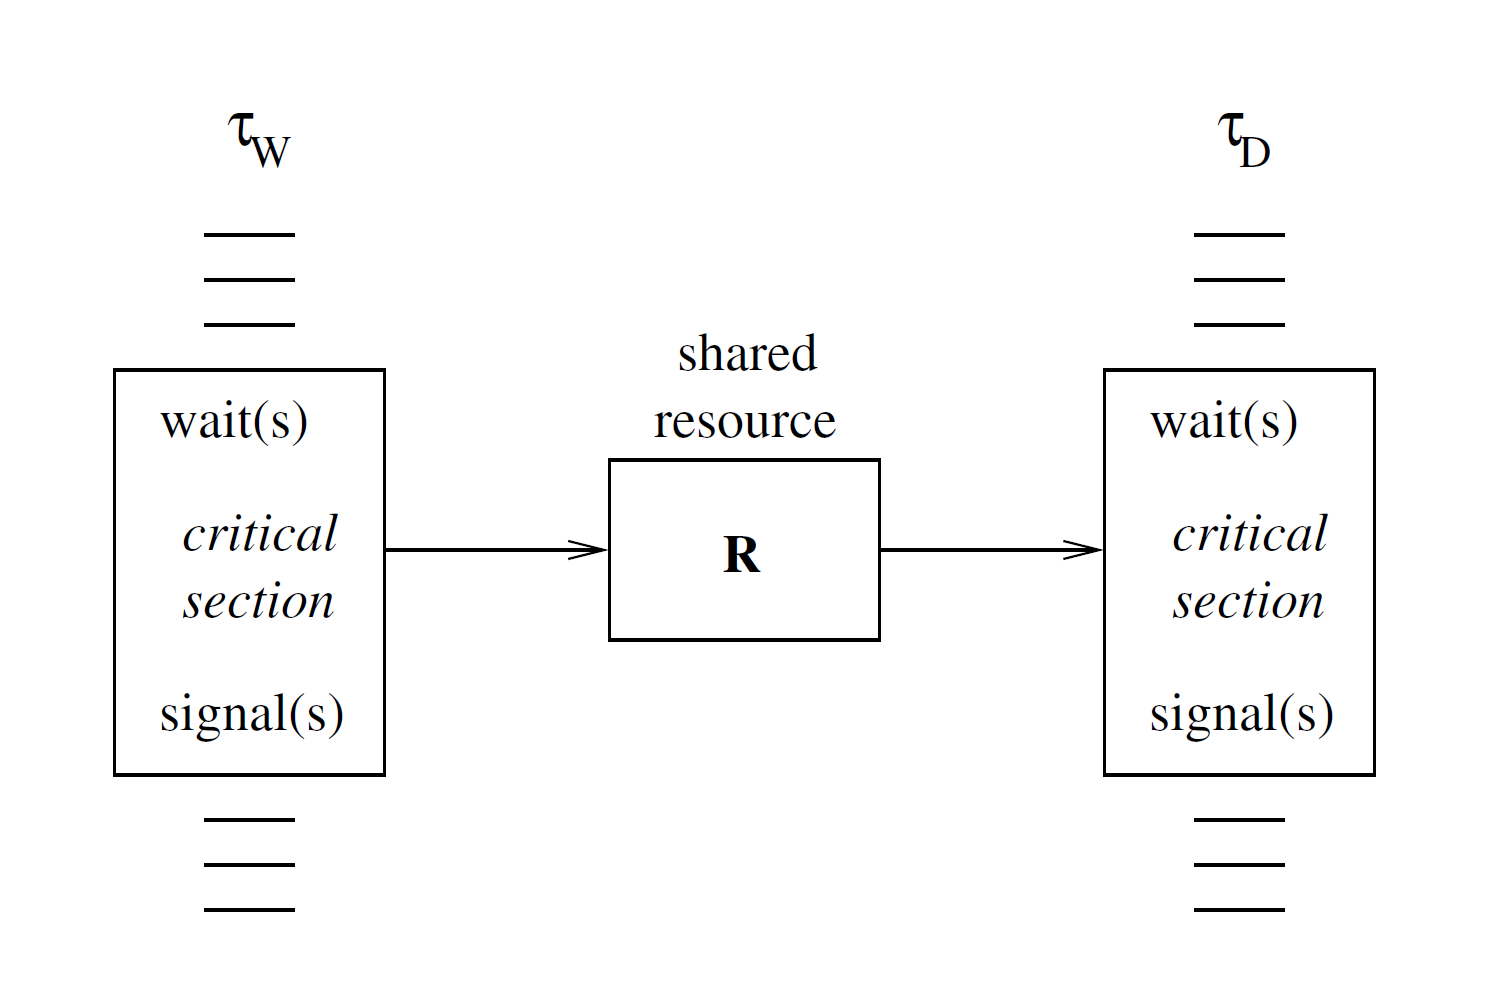
\includegraphics[width=0.60\textwidth]{pictures/strutturaSezioneCritica.png}
    \caption{Struttura di due task che accedono a una risorsa condivisa in mutua esclusione, tramite meccanismo di semafori}
\end{figure}
\begin{figure}[H]
    \centering
    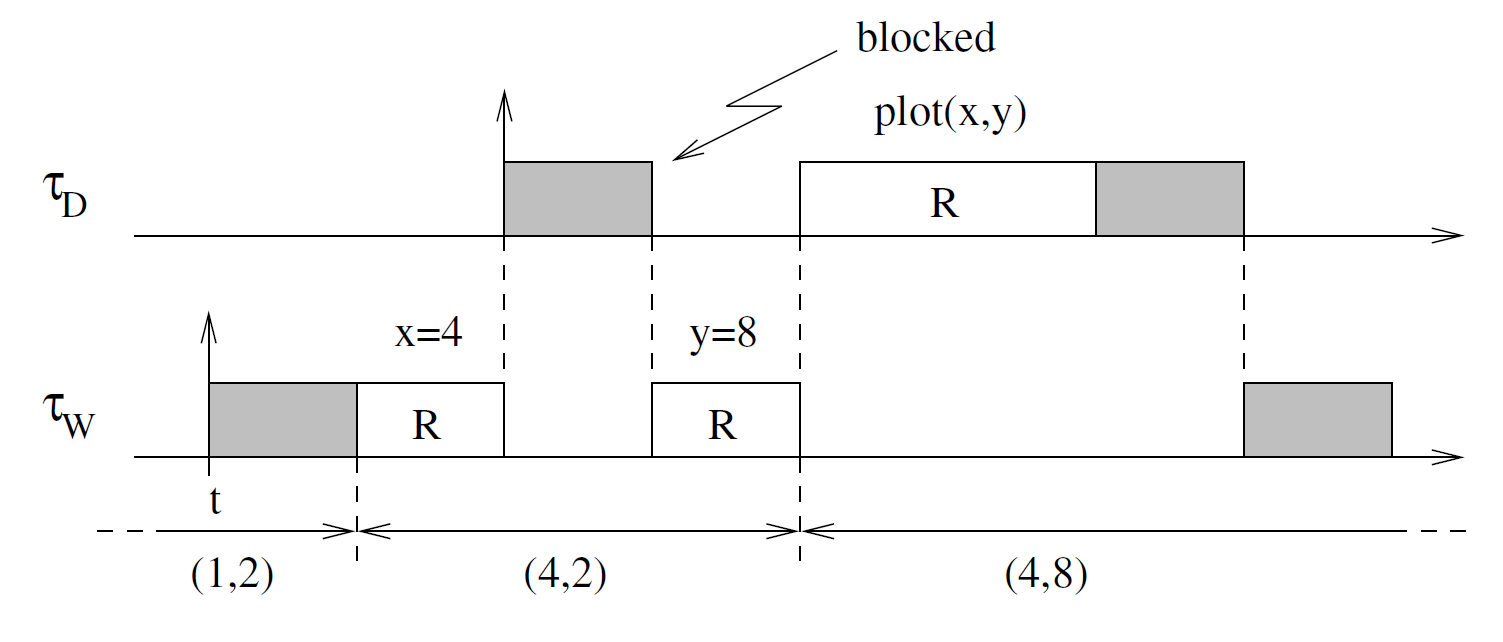
\includegraphics[width=0.75\textwidth]{pictures/schedulingCorsaCritica.png}
    \caption{Esempio di scheduling quando la risorsa è protetta da un semaforo}
\end{figure}
\begin{figure}[H]
    \centering
    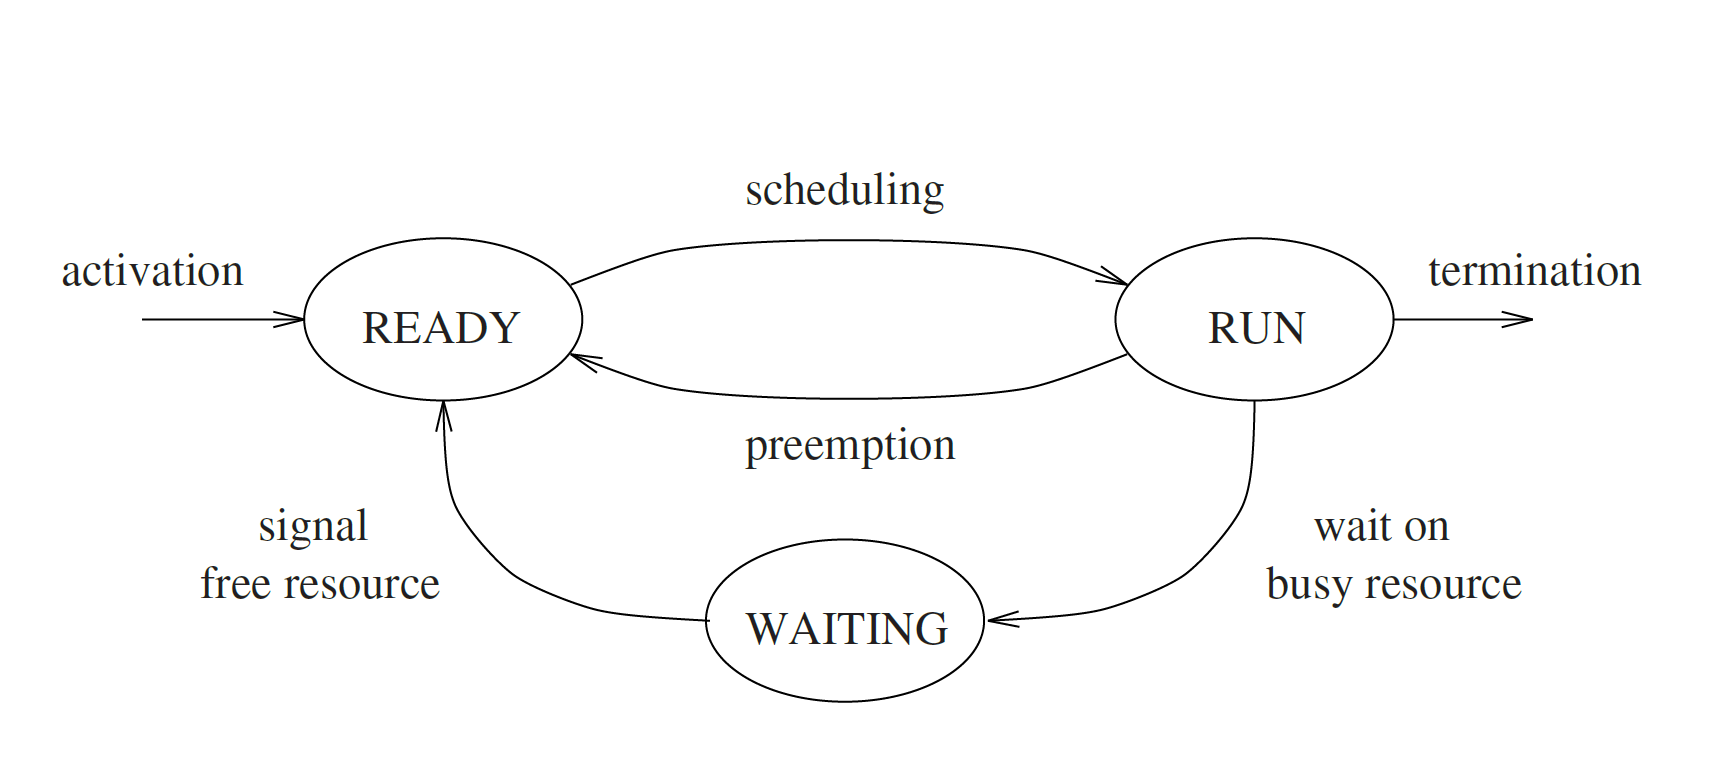
\includegraphics[width=0.75\textwidth]{pictures/cicloWait.png}
    \caption{Stato di wait causato da un vincolo sulle risorse}
\end{figure}
\noindent Quando un task è in attesa di una risorsa condivisa, si dice che è \textit{bloccato} su quella risorsa.
Tutti i task bloccati su una stessa risorsa vengono messi in una \textbf{wait queue} associata a un semaforo che protegge la risorsa.
Quando un task in esecuzione utilizza la primitiva \textit{wait} su un semaforo bloccato, entra nello stato di \textbf{wait}, fino a quando un altro task non esegue la primitiva \textit{signal} che sblocca il semaforo.
Nota che quando un task lascia lo stato di wait non entra immediatamente nello stato di running, ma entra nello stato di ready, cosicché la CPU possa essere assegnata a un task con priorità più alta dall'algoritmo di scheduling.

\subsection{Classificazione di algoritmi di scheduling}
Le classi principali di algoritmi di scheduling sono:
\begin{itemize}
    \item \textbf{Preemptive vs. non preemptive}
    \begin{itemize}
        \item Preemptive: un task può essere interrotto in qualsiasi momento da un task con priorità più alta, secondo una policy di scheduling definita in precedenza.
        \item Non preemptive: un task una volta avviato deve essere eseguito fino al termine della sua esecuzione. Tutte le scelta di scheduling vengono effettuate quando il task termina la sua esecuzione.
    \end{itemize}
    \item \textbf{Static vs. Dynamic}
    \begin{itemize}
        \item Static: le decisioni di scheduling avvengono in base a un insieme di parametri che vengono definiti prima dell'attivazione dei task.
        \item Dynamic: le decisioni di scheduling avvengono in base a un insieme di parametri che possono essere modificati durante l'evoluzione del sistema.
    \end{itemize}
    \item \textbf{Off-line vs. online} 
    \begin{itemize}
        \item Off-line: Le decisioni di scheduling vengono interamente prese per l'intero insieme di task prima dell'attivazione di essi.
        Questo scheduling è memorizzato in una tabella e successivamente viene eseguito dal dispatcher.
        \item Online: Le decisioni di scheduling vengono prese a runtime ogni volta che un nuovo task entra nel sistema, o quando un task running termina. Notare che questo genera un overhead.
    \end{itemize}
    \item \textbf{Ottimale vs. euristico}
    \begin{itemize}
        \item Ottimale: Un algoritmo è detto ottimale se minimizza la "funzione costo" definita per l'insieme di task.
        Quando non è definita questa funzione costo il nostro unico obiettivo è ottenere uno schedule feasible (se esiste).
        \item Euristico: Un algoritmo è detto euristico se è guidato da una funzione euristica per prendere decisioni di scheduling.
        Un algoritmo euristico tende verso lo scheduling ottimale, ma non è garantito che lo raggiunga.
    \end{itemize}
\end{itemize}
Inoltre un algoritmo è detto \textit{chiaroveggente} se conosce il futuro, ovvero conosce in anticipo il tempo di arrivo di tutti i task. Questo algoritmo chiaramente non esiste, ma è utilizzato come benchmark per valutare gli altri algoritmi in confronto al caso perfetto.
\subsubsection{Algoritmi di scheduling basati sulla garanzia}
Nelle applicazioni hard real-time sono richiesti comportamenti altamente predicibili, la feasibility di uno scheduling dovrebbe essere garantita in anticipo (prima dell'attivazione dei task).
In questa maniera, così che se un task critico non può essere schedulato prima della sua deadline, il sistema è in tempo per eseguire un'azione alternativa che tenta di evitare conseguenze catastrofiche.
Per controllare la feasibility di uno scheduling prima dell'esecuzione dei task il sistema deve pianificare le sue azioni assumendo il caso peggiore.
Quindi vanno analizzati i parametri del task set per verificare che esista uno scheduling ammissibile.
Nei sistemi statici, ovvero il task set è fisso e noto a priori, tutte le attivazioni dei task possono essere pre calcolate off-line, e tutto lo schedule può essere memorizzato in una tabella che contiene tutti i task garantiti.
Poi a runtime il dispatcher può semplicemente eseguire lo schedule memorizzato. Il vantaggio principale dell'approccio statico è che l'overhead a runtime non dipende dalla complessità dell'algoritmo di scheduling.
Questo permette di utilizzare algoritmi di scheduling sofisticati per risolvere problemi complessi. D'altro canto, il sistema è rigido rispetto a cambiamenti nell'ambiente.\\
Nei sistemi dinamici (che tipicamente consistono di task \textit{firm}) i task possono essere creati a runtime, dunque la garanzia di scheduling deve essere effettuata online ogni volta che un nuovo task viene creato.
\begin{figure}[H]
    \centering
    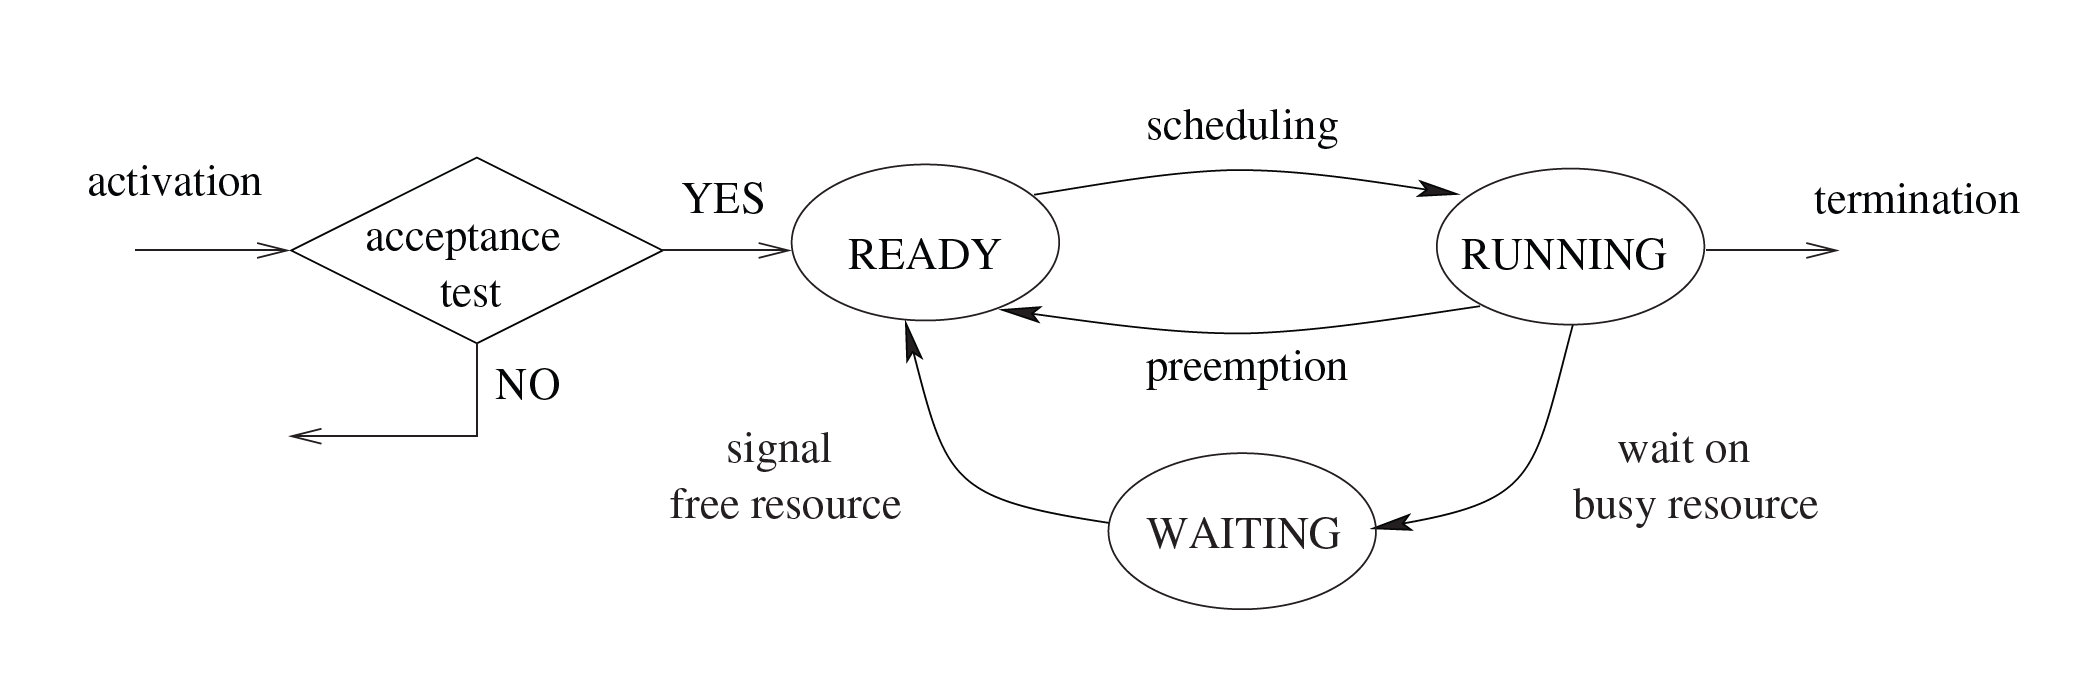
\includegraphics[width=\textwidth]{pictures/garanziaDinamica.png}
    \caption{Meccanismo di garanzia in un sistema dinamico real time}
\end{figure}
\noindent Inoltre deve essere garantito che quando un task viene accettato, esso non deve interdire la feasibility di task garantiti in precedenza.
\subsubsection{Algoritmi di scheduling best effort}
Nelle applicazioni real-time soft, i task non hanno vincoli temporali stringenti, ma devono essere eseguiti in un tempo ragionevole per soddisfare i requisiti si sistema.
Dunque il mancato rispetto delle deadline non porta a conseguenze catastrofiche, ma porta a una degradazione delle performance.
Un algoritmo best effort cerca di fare "del suo meglio" per rispettare le deadline, ma non garantisce di trovare uno scheduling feasible.
Negli approcci best effort i task potrebbero essere messi in coda in base a delle politiche che considerano i requisiti temporali, ma non viene controllata la feasibility e quindi un task potrebbe venir abortito durante la sua esecuzione.\\
Mediamente le performance di un algoritmo best effort sono migliori rispetto a quelle di un algoritmo basato sulla garanzia, infatti un algoritmo basato sulla garanzia
potrebbe, basandosi sul caso peggiore, rifiutare inutilmente un task che in realtà sarebbe riuscito a rispettare la deadline.

\section{Scheduling di task aperiodici}
Gli algoritmi affrontati in questa sezione riguardano task aperiodici real-time, eseguiti su una macchina single core.
Ogni algoritmo è una soluzione a un problema di scheduling espresso come insieme di assunzioni sulle task e criteri di ottimalità da utilizzare.
Pur essendo pensati per task aperiodici su macchine monoprocesso, molti di questi algoritmi possono essere estesi per lavorare su sistemi multiprocessore o architetture distribuite per lavorare con task set più complessi.
\\
Per descrivere un problema di scheduling utilizziamo i parametri $\alpha|\beta|\gamma$:
\begin{itemize}
\item $\alpha$ è il tipo di macchina (uniprocessore, multiprocessore, distribuito, ecc.)
\item $\beta$ descrive le task e le caratteristiche delle risorse (preemptive, indipendente vs vincoli di precedenza, attivazione asincrona, etc.)
\item $\gamma$ è il criterio di ottimalità
\end{itemize}
\subsection{Garanzie}
Per garantire che esista uno scheduling feasible dobbiamo mostrare che, nel caso peggiore, tutti i task vengano completati prima delle rispettive deadline.
Vale a dire che per ogni task dobbiamo mostrare che il tempo di completamento nel caso peggiore $f_i$ è minore o uguale alla rispettiva deadline $d_i$.
\begin{equation}
    f_i \leq d_i , \forall i \in \{1,2,\ldots,n\}
\end{equation}
Se un task ha requisiti hard, quest'analisi di fattiblità deve essere effettuata prima dell'esecuzione dei task.
Senza perdita di generalità possiamo assumere che i task $J_1,J_2,\dots J_n$ siano elencati in ordine di deadline crescente, ovvero $J_1$ ha la deadline più vicina.
In questo caso il tempo di completamento del task $J_i$ nel caso peggiore è dato da:
\begin{equation}
    f_i=\sum_{k=1}^{i} C_k
\end{equation}
Dunque in un task set con $n$ task il test di garanzia consiste nel verificare che:
\begin{equation}
    \forall i \in \{1,2,\dots ,n\} \sum_{k=1}^i C_j \leqq d_i
\end{equation}
\subsection{Earliest Deadline First (EDF)}
Se le task non sono sincrone ma possono avere tempo di arrivo arbitrario, la preemption diventa un fattore importante.
In generale un problema di scheduling dove la preemption è permessa è sempre più facile da risolvere rispetto allo stesso problema senza preemption.
Una soluzione elegante a problemi del tipo $1|preem|L_{max}$ è data dall'algoritmo \textbf{Earliest Deadline First} (EDF).
\begin{theorem}
    Dato un insieme di $n$ task con tempo di arrivo arbitrario, ogni algoritmo che a ogni istante esegue il task con la deadline assoluta più vicina tra tutti i task attivi è ottimale rispetto alla minimizzazione della lateness.
\end{theorem}
La complessità computazionale dell'algoritmo è $O(n)$ per ogni task se la ready queue è implementata come lista, e $O(\log n)$ se la ready queue è implementata come heap.
Da notare che EDF non fa assunzioni esplicite sulla periodicità dei task, dunque può essere usato sia per task set aperiodici che per task set periodici.

\subsubsection{Garanzia}
Quando i task hanno attivazioni dinamiche e il tempo di arrivo non è noto a priori, il test di garanzia deve essere fatto dinamicamente ogni volta che un task entra nel sistema.
Sia $\mathcal{T}$ l'insieme corrente di task attivi, che sono stati garantiti in precedenza, sia $J_{new}$ il nuovo task che entra nel sistema.
Per poter accettare $J_{new}$ dobbiamo garantire che il nuovo task set $\mathcal{T} \cup J_{new}$ sia schedulabile.\\
Sotto le assunzioni di \ref{assunzioni} possiamo verificare la schedulabilità di un task set periodico con EDF attraverso il fattore di utilizzo del processore.
In questo caso $U_{lub}=1$, quindi un task potrebbe usare il 100\% della CPU ed essere schedulabile.
\begin{theorem}
    Un task set di task periodici è schedulabile da EDF se e solo se:
    \begin{equation}
        \sum_{i=1}^{n}\frac{C_i}{T_i}\leq 1
    \end{equation}
\end{theorem}
\subsection{EDF con vincoli di precedenza}
Consideriamo problemi di scheduling del tipo $1|prec,preem|L_{max}$, dove i task sono soggetti a vincoli di precedenza.
Il problema di schedulare un insieme di n task con vincoli di precedenza con attivazioni dinamiche può essere risolto in tempo polinomiale \underbar{SOLO} se i task sono preentable.
L'idea alla base dell'approccio è quella di trasformare  il set di task dipendenti $\mathcal{T}$ in un insieme di task indipendenti $\mathcal{T}^*$ tramite adeguate modifiche ai parametri temporali, dopodiché possiamo applicare l'algoritmo EDF.
L'algoritmo di trasformazione garantisce che $\mathcal{T}$ sia schedulabile se e solo se $\mathcal{T}*$ è schedulabile. In pratica tutti i release time e le deadline sono modificati in modo che ogni task non possa cominciare prima del predecessore e non possa fare preemption su i suoi successori.

\section{Scheduling di task periodici}
In molti sistemi real-time di controllo, le attività periodiche compongono la maggior parte della computazione del sistema.
Quando una applicazione di controllo consiste in molteplici task periodici concorrenti, con vincoli temporali indipendenti, il sistema operativo deve garantire che ogni istanza periodica 
venga regolarmente attivata con la giusta frequenza e che venga eseguita entro la deadline (che in generale è diversa dal suo periodo).\\
Per semplificare l'analisi di scheduling vengono assunte le seguenti ipotesi:
\begin{enumerate}
    \label{assunzioni}
    \item Le istanze di task periodici $\tau_i$ sono regolarmente attivate a frequenza costante, ovvero ogni $T_i$ (periodo del task).
    \item Tutte le istanze di un task periodico $\tau_i$ hanno lo stesso WCET $C_i$.
    \item Tutte le istanze di un task periodico $\tau_i$ hanno la stessa deadline relativa $D_i$, che è uguale a $T_i$.
    \item Tutte le task di $\mathcal{T}$ sono indipendenti.
\end{enumerate}
Inoltre alcune assunzioni implicite sono:
\begin{itemize}
    \item Nessun task si può bloccare da solo, ad esempio per operazioni di I/O.
    \item Tutti i task vengono rilasciati appena arrivano nel sistema.
    \item L'overhead del kernel viene considerato nullo.
\end{itemize}
Per quest'ultima assunzione potrei evitare problemi se considero solo una percentuale di "potenza di cpu" disponibile, così da lasciare dello spazio per l'overhead del kernel.\\
Nota che le prime due assunzioni non sono restrittive, dato che in molte applicazioni di controllo ogni attività periodica richiede l'esecuzione della stessa routine a intervalli regolari.
Quando si analizzano casi realistici, le assunzioni 3 e 4 vengono rilassate.
\\
Altri parametri importanti per i task periodici sono:
\begin{itemize}
    \item \textbf{Hyperperiod}: minimo intervallo di tempo nel quale lo scheduling si ripete.
    \item \textbf{Critical instant} di un task: tempo di arrivo che produce il response time del task più lungo.
\end{itemize}
\subsection{Fattore di utilizzo del processore}
Dato un insieme di task periodici $\Gamma$, il \textit{fattore di utilizzo} del processore $U$ è la frazione del tempo di CPU che viene utilizzato per eseguire l'insieme di task.
Dato che $\frac{C_i}{T_i}$ è la frazione di tempo di CPU utilizzata da un task $\tau_i$, il fattore di utilizzo del processore è dato da:
\begin{equation}
    U = \sum_{i=1}^{n} \frac{C_i}{T_i}
\end{equation}
Questo valore ci fornisce una misura del carico computazionale sulla CPU. Nonostante possa essere migliorato aumentando il tempo di computazione dei task o diminuendo il loro periodo, esiste un valore massimo 
di $U$ per il quale $\Gamma$ è schedulabile. Tale limite dipende dalla relazione dei periodi dei task e dall'algoritmo di scheduling utilizzato.
Sia $U_{ub}(\Gamma,A)$ il limite superiore al fattore di utilizzo del processore per un insieme di task $\Gamma$ schedulato con l'algoritmo $A$.
Quando $U = U_{ub}(\Gamma,A)$, si dice che $\Gamma$ \textit{utilizza completamente} il processore. In questo caso $\Gamma$ è schedulabile da $A$, ma un qualsiasi aumento nel tempo di computazione rende il task set non feasible.
Per un algoritmo di scheduling $A$, il limite superiore minore $U_{lub}(\Gamma,A)$ è il minimo fattore di utilizzo su tutti i task set che utilizzano completamente il processore.
\begin{equation}
    U_{lub}(\Gamma,A) = \min_{\Gamma } U_{ub}(\Gamma,A)
\end{equation}
Dato che $U_{lub}(\Gamma,A)$ è il minimo di tutti gli upper bound, qualsiasi task set con fattore di utilizzo minore di $U_{lub}(\Gamma,A)$ è \underline{sicuramente} schedulabile da $A$. In questa maniera 
è facilmente determinabile se un task set è schedulabile o meno con un determinato algoritmo. 
\begin{itemize}
    \item Se $ U_{lub}< U < 1.0$, la schedulabilità viene raggiunta solo se i periodi sono compatibili.
    \item Se $U_{lub} > 1.0 $, il task set \underline{non è schedulabile da nessun algoritmo}.
\end{itemize}
\subsection{Timeline scheduling}
Anche noto come \textit{Cyclic Executive}, è uno degli approcci più adottati per gestire task periodici nei sistemi di difesa militari e di controllo di traffico.
Il metodo consiste nel dividere l'asse temporale in slot di egual lunghezza, nei quali uno o più task vengono allocati per l'esecuzione; in modo da rispettare le frequenze date dai requisiti.
Un timer sincronizza l'attivazione dei task all'inizio di ogni slot.\\
Consideriamo un esempio dove tre task $A,B$ e $C$ devono essere eseguiti con frequenze rispettivamente di $40Hz$, $20Hz$ e $10Hz$.
Dunque i rispettivi periodi sono $T_A=25ms$, $T_B=50ms$ e $T_C=100ms$ (N.B. $F=\frac{1}{T}$), si ricava che la lunghezza ottimale dello slot è di 
$25ms$, che è il massimo comune divisore dei periodi. Quindi il task $A$ viene eseguito ogni slot, il task $B$ ogni 2 slot e il task $C$ ogni 4 slot.
\begin{figure}[H]
    \centering
    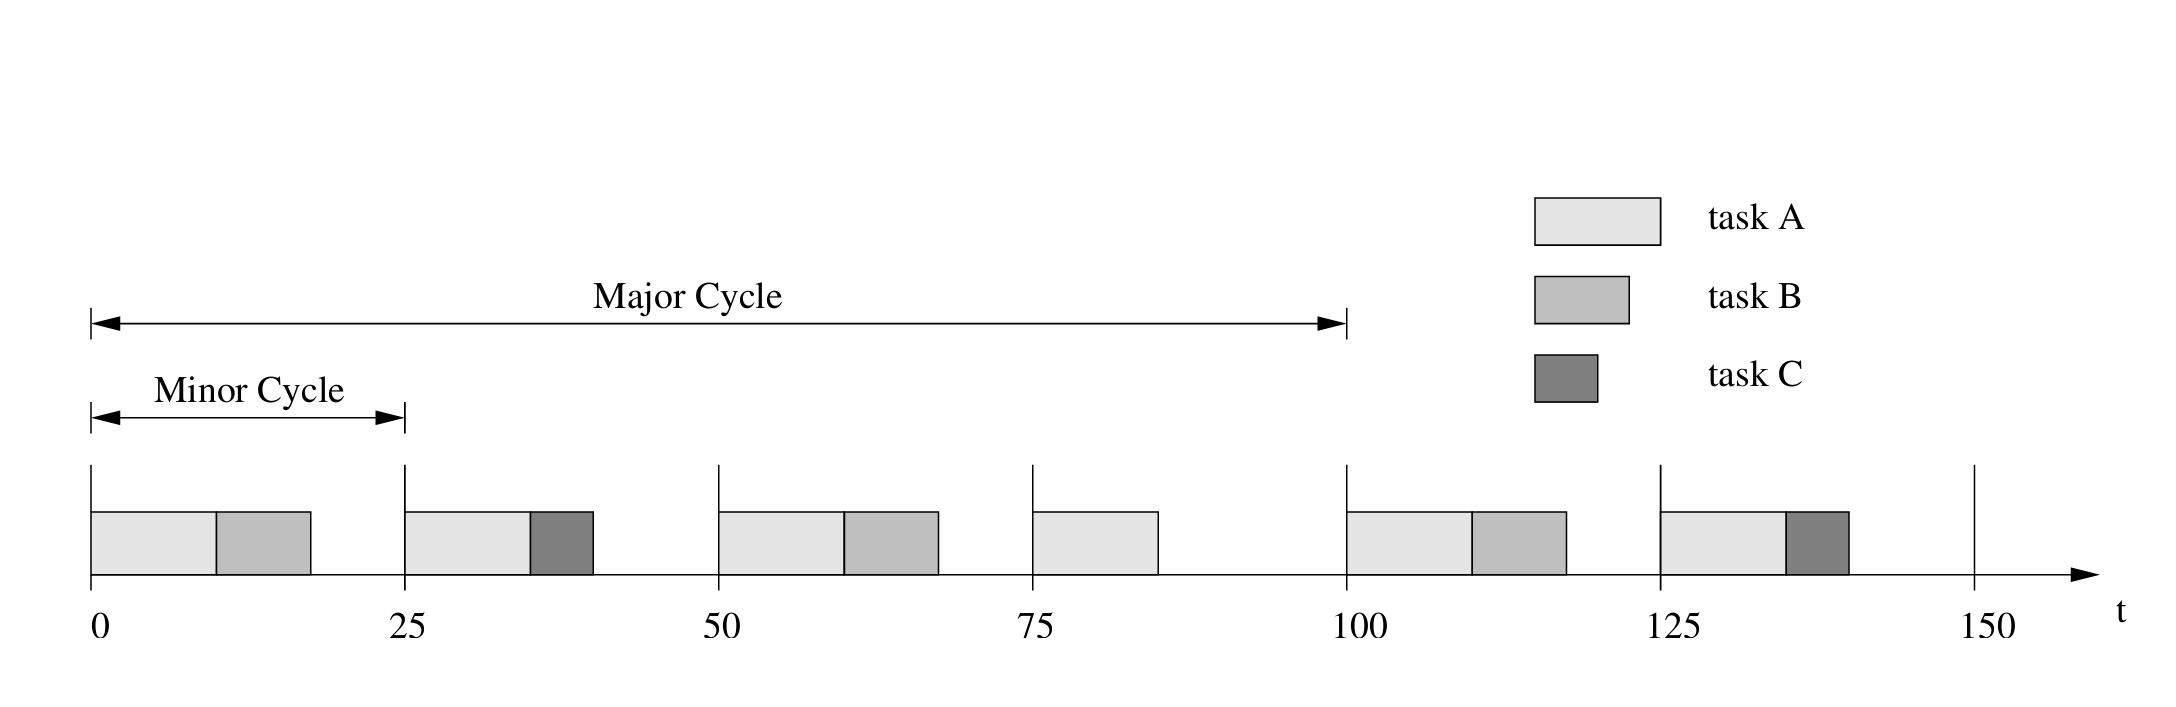
\includegraphics[width=\textwidth]{pictures/timelineScheduling.png}
    \caption{Esempio di timeline scheduling}
\end{figure}
\noindent La durata dello slot è detta \textit{Minor cycle}, mentre l'intervallo minio di tempo dopo il quale uno schedule si ripete è detto \textit{Major cycle}.
\\
In generale, il major cycle è uguale al minimo comune multiplo di tutti i periodi. Per poter garantire a priori che lo schedule sia feasible su un processore,
è sufficiente sapere il WCET dei task e verificare che la somma all'interno di ogni slot sia minore o uguale al minor cycle.
\\
Il \textbf{vantaggio} principale di timeline scheduling è la sua \textbf{semplicità}. Può essere implementato tra programmando un timer che interrompa con periodo uguale al minor cycle
e scrivendo un ciclo main dove i task vengono chiamati nell'ordine dato dal major cycle, inserendo punti di sincronizzazione a ogni inizio del minor cycle.
Dato che la sequenza di attivazione dei task non è determinata da un algoritmo di scheduling nel kernel, ma è determinata dalle chiamate effettuate dal main, non vi sono context switch, dunque l'overhead a runtime è molto basso.
Nonostante questi vantaggi, vi sono dei problemi, ad esempio l'alta fragilità in situazioni di overload. Se un task non termina nel limite del minor cycle, può essere continuato o abortito.
In entrambi i casi, il sistema entra in uno stato critico.
Se il task fallimentare rimane in esecuzione esso può causare un effetto a domino sugli altri task, rompendo l'intero schedule (timeline break).
Se un task viene abortito mentre compie azioni su risorse condivise, esso può lasciare le risorse in uno stato inconsistente e causare un comportamento non corretto.
Inoltre è particolarmente sensibile a cambiamenti nei requisiti.
\subsection{Rate Monotonic Scheduling (RMS)}
Funziona tramite una semplice regola che assegna la priorità a un task in base alla sua frequenza di attivazione.
In particolare, task con periodi più brevi hanno priorità più alta.
Dato che i periodi sono costanti, RM è un sistema fixed priority, ovvero la priorità $P_i$ di un task $i$ non cambia durante l'esecuzione.
RM è intrinsecamente preemptive, ovvero un task con priorità più alta può interrompere un task con priorità più bassa.
È stato dimostrato da Liu e Layland che RM è ottimale rispetto a tutti gli assegnamenti di priorità fissi, nel senso che nessun altro sistema di scheduling a priorità fissa può schedulare un task set che non può essere schedulato da RM.
\\
Liu e Layland hanno inoltre derivato che $U_{lub}$ per RM su un task set di $n$ task è dato da:
\begin{equation}
    U_{lub} = n(2^{\frac{1}{n}}-1)
\end{equation}
\begin{table}[H]
    \centering
    \subfloat[]{ 
        \begin{tabular}{|l|l|}
        \hline
        n & $U_{lub}$ \\ \hline
        1 & 1.000 \\ \hline
        2 & 0.828 \\ \hline
        3 & 0.780 \\ \hline
        4 & 0.757 \\ \hline
        5 & 0.743 \\ \hline
        \end{tabular}
    }
    \qquad
    \subfloat[]{ 

        \begin{tabular}{|l|l|}
        \hline
        n  & $U_{lub}$      \\ \hline
        6  & 0.73  \\ \hline
        7  & 0.729 \\ \hline
        8  & 0.724 \\ \hline
        9  & 0.721 \\ \hline
        10 & 0.718 \\ \hline
        \end{tabular}
    } 
    \caption{Valori di $U_{lub}$ per RM al variare di n} 
\end{table}
\noindent
Il bound diminuisce all'aumentare di $n$. Per valori alti $U_{lub}$ converge a $U_{lub} = \ln 2 \approx 0.69$. 
\subsubsection{Bound iperbolico per RM}
L'analisi di fattibilità su RM può anche essere effettuata utilizzando un bound iperbolico.
Il test ha la stessa complessità computazionale di quello di Liu e Layland, ma è meno pessimistico, dato che accetta task se4t che verrebbero rifiutati dal test LL.
Il seguente teorema offre una condizione sufficiente per testare la schedulabilità di un task set con RM.
\begin{theorem}
    
    Sia $\Gamma=\{\tau_1,\tau_2,\dots,\tau_n\}$ un insieme di task periodici dove ogni task $\tau_i$ è caratterizzato dal fattore di utilizzo $U_i$. Allora $\Gamma$ è schedulabile da RM se:
    \begin{equation}
        \label{eq:boundIperbolico}
        \prod_{i=1}^{n}(U_i+1) \leq 2
    \end{equation}
\end{theorem}
Rappresentiamo in un piano $n$ dimensionale il bound LL che interseca gli assi in $U_{lub}=n(2^{\frac{1}{n}}-1)$.
Tutti i punti al di sotto la superficie di RM rappresentano task set periodici schedulabili da RM.
Il nuovo bound viene rappresentato da una superficie iperbolica tangente al piano RM e che interseca gli assi in $U_i=1$.
Rappresentiamo in figura il bound iperbolico per $n=2$. Da notare che gli asintoti dell'iperbole sono a $U_1=-1$.
Dal plot possiamo notare che la regione di ammissibilità è più grande per il test H-bound che per il test LL.
\begin{figure}[H]
    \centering
    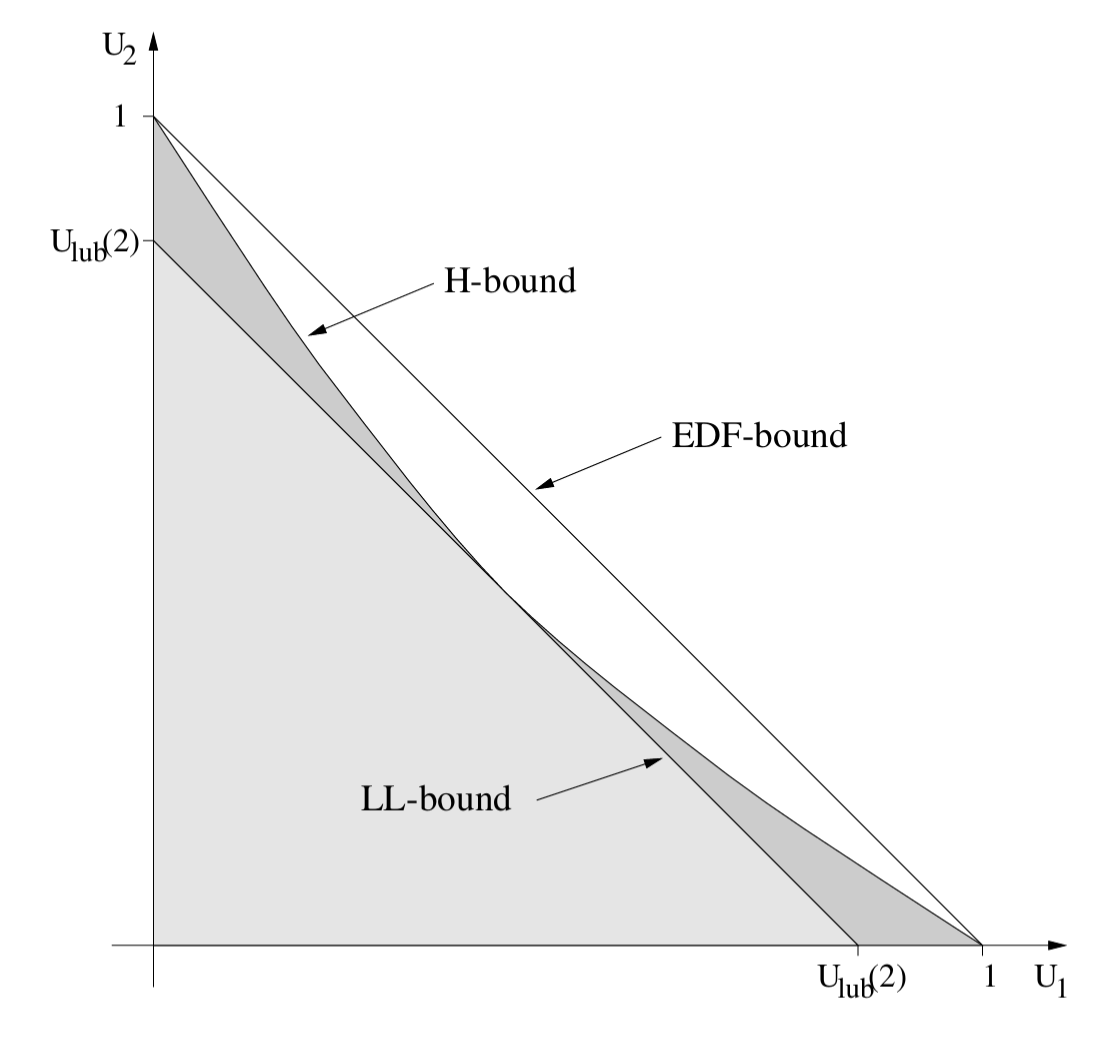
\includegraphics[width=0.5\textwidth]{pictures/boundIperbolico.png}
    \caption{Bound iperbolico per RM con $n=2$}
\end{figure}
\subsection{RM vs EDF}
Il problema di schedulare un insieme di task periodici indipendenti e preemptable è stato risolto sia con sistemi a priorità fissa (RM) che con sistemi a priorità dinamica (EDF).
Il vantaggio principale di sistemi a priorità fissa è la semplicità di implementazione, inoltre se la ready queue è implementata come una queue multi livello con $P$ livelli di priorità,
sia l'inserimento che la rimozione di un task dalla ready queue richiede $O(1)$ tempo.
\\
D'altro canto in uno scheduler deadline driven, la soluzione migliore è l'implementazione tramite heap, dove l'inserimento e la rimozione richiedono $O(\log n)$ tempo.
Per quanto riguarda l'utilizzo del processore, EDF è in grado di utilizzare completamente la CPU, mentre RM può garantire la fattibilità di task set con fattore di utilizzo minore al 69\% nel caso peggiore.
\\
Nonostante la computazione maggiore richiesta da EDF per aggiornare le deadline assoluta a ogni attivazione di task, EDF introduce meno overhead a runtime quando vengono considerati i context switch.
Infatti, per applicare l'ordine a priorità fissa, il numero di preemption che tipicamente si verifica con RM è \textit{molto maggiore} rispetto a EDF.
\\
Una proprietà interessante di EDF durante overload permanenti è che viene performata in automatico un riscalaggio dei periodi, così che si comportino come se venissero eseguiti a frequenza più bassa, questo fenomeno viene chiamato \textbf{graceful degradation} e deve essere evitato.
Come verrà discusso in seguito, un altro grande vantaggio dello scheduling dinamico rispetto ai sistemi a priorità fissa è una migliore responsività nel gestire task aperiodici.
Questa proprietà deriva dal fattore di utilizzo del processore maggiore in EDF, infatti il bound minore di RM limita l'utilizzo massimo che può essere assegnato a un server per garantire la schedulabilità di un task set periodico.
Di conseguenza l'utilizzo di processore che avanza che non può essere assegnata al server viene sprecata come esecuzione di background.
Questo non avviene con EDF.
\section{Server a priorità fissa}
Gli algoritmi di scheduling trattati in precedenza lavorano su task set omogenei, dove tutti le attività computazionali sono periodiche o aperiodiche.
Nella realtà dei fatti nelle applicazioni di controllo real time i due tipi si possono mischiare, avendo anche diversi livelli di criticità.
Tipicamente i task periodici sono time-driven ed eseguono attività di controllo critiche con vincoli di temporizzazione hard con lo scopo di garantire la attivazione regolare dei task.
Quando i task set sono ibridi lo scopo principale del kernel è di garantire la schedulabilità di tutti i task critici nel caso peggiore, e di offrire buoni response time per gli altri.
Tutti gli algoritmi che verranno trattati in questa sezione sono basati sulle seguenti assunzioni:
\begin{itemize}
    \item I task periodici sono schedulati tramite RM (fixed priority).
    \item Tutti i task periodici iniziano a $t=0$ e le loro deadline relative sono uguali al loro periodo.
    \item Il tempo di arrivo dei task aperiodici è arbitrario.
    \item Quando non viene specificato, il minimo tempo di "interarrivo" di un task periodico è uguale alla sua deadline.
    \item \textbf{Tutti} i task sono preemptable.
\end{itemize}
\subsection{Background scheduling}
\label{sec:backgroundScheduling}
È il metodo più semplice per gestire task aperiodici soft in presenza di task periodici, consiste nel schedulare i task aperiodici quando non ci sono istanze di task periodici in stato di ready.
Il problema principale di questo approccio è che, per carichi periodici elevati, il response time delle richieste aperiodiche può essere troppo lungo per alcune applicazioni.
Per questo motivo background scheduling può essere adottato solo quando le attività aperiodiche non hanno vincoli di temporizzazione stringenti e il carico di lavoro periodico è basso.
\begin{figure}[H]
    \centering
    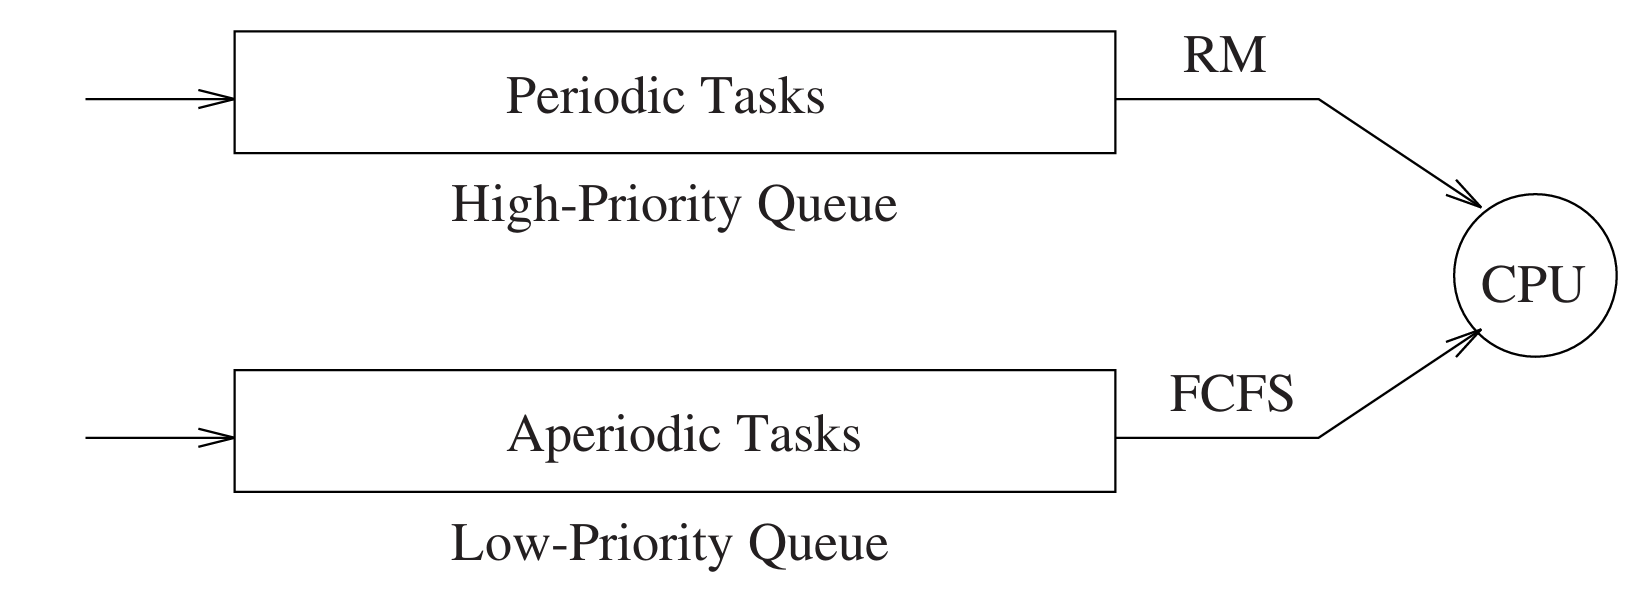
\includegraphics[width=0.8\textwidth]{pictures/backgroundScheduling.png}
    \caption{Esempio di ready queue per background scheduling}  
    \label{fig:backgroundScheduling}
\end{figure}
\noindent
Il vantaggio principale di background scheduling è la sua semplicità.
Da notare che come mostrato in figura \ref{fig:backgroundScheduling}, le due strategie di attesa dei task sono indipendenti e possono essere realizzate con algoritmi differenti.
L'attivazione di un nuovo task periodico causa la preemption di un qualsiasi task aperiodico.

\subsection{Polling server}
\label{sec:pollingServer}
Il tempo di risposta medio di task aperiodici può essere migliorato rispetto a background scheduling attraverso l'utilizzo di un \textbf{server}, ovvero, un task periodico il quale scopo è di servire task aperiodici non appena possibile.
Come qualsiasi task periodico, il server ha un periodo $T_s$ e un tempo di computazione $C_s$, detto anche \textit{capacità} o \textit{budget}.
In generale, il server viene schedulato con lo stesso algoritmo usato per gli altri task periodici e, una volta attivo, serve i task aperiodici nel limite del suo budget.
Da notare che l'ordine in cui vengono serviti i task aperiodici non è determinato dall'algoritmo usato per quelli periodici.
\\
Il polling server a intervalli regolari $T_s$  diventa attivo ed esegue task aperiodici nel limite del suo budget $C_s$.
Se nessun task aperiodico è in attesa, il server si sospende fino al prossimo periodo e il budget viene lasciato a task periodici.
\subsubsection{Dare una dimensione a un server polling}
Dato un set di task periodici, come possiamo computare $T_s$ e $C_s$ in maniera da avere uno schedule feasible?
Prima di tutto calcoliamo il fattore massimo di utilizzo del server $U_s^{max}$, che garantisce la feasibility del task set.
Dato che il response time non è facile da manipolare a causa di arrotondamenti, possiamo derivare $U_s^{max}$ dal test iperbolico \ref{eq:boundIperbolico}, che è più restrittivo rispetto al test di LL.
definiamo:
\begin{equation}
    P \stackrel{\mathrm{def}}{=} \prod_{i=1}^{n}(U_i+1)
\end{equation}
allora dobbiamo avere 
\begin{equation}
    P \leq \frac{2}{U_s+1}
\end{equation}
ovvero
\begin{equation}
    U_s \leq \frac{2-P}{P}
\end{equation}
dunque 
\begin{equation}
    U_s^{max} = \frac{2-P}{P}
\end{equation}
Quindi $U_s$ deve essere minore di $U_s^{max}$. Per un dato $U_s$ ci sono infinite coppie $(C_s,T_s)$, quindi ne dobbiamo selezionare una.
Una soluzione semplice è assegnare al server la priorità più alta (e quindi in RM con il periodo più breve), però non è utile avere $T_s<T_1$. dato che un piccolo $T_s$ implica un minore $C_s$ e questo causerebbe una maggiore frammentazione (quindi runtime overhead per i cambi di contesto).
\subsection{Deferrable server}
\label{sec:deferrableServer}
Pensato per migliorare i response time per task aperiodici rispetto polling server.
La differenza è che se nessun task aperiodico è in attesa, il server non si sospende e rimane in attesa (continuando a consumare il budget) fino a quando un task aperiodico non entra nella ready queue e, compatibilmente con il budget rimanente, lo esegue.
La capacità viene ricaricata all'inizio di ogni periodo.
DS offre una risposta molto più rapida rispetto al PS, dato che preserva la capacità fino a quando server.
Tempi di risposta più rapidi possono essere ottenuti dando a DS la priorità più alta tra i task periodici.
\subsection{Priority exchange}
\label{sec:priorityExchange}
Pensato per servire un insieme di task aperiodici soft in presenza di task periodici hard.
Rispetto a PS e DS è leggermente meno performante in termini di risposta a task aperiodici, ma offre migliori bound di schedulabilità per insiemi di task periodici.
Come DS e PS utilizza un server periodico (tendenzialmente con alta priorità), con la differenza rispetto DS che riserva la sua capacità ad alta priorità scambiandola con tempo di esecuzione di task periodici a priorità più bassa.
All'inizio di ogni periodo del server la capacità viene ricaricata. Se dei task aperiodici sono in attesa e il server è il task ready con priorità più alta, allora le richieste vengono servite consumando la capacità, altrimenti $C_s$ viene scambiato con tempo di esecuzione di un task periodico con la priorità più alta.
\\
\textbf{Quando uno scambio di priorità avviene il task periodico viene eseguito con il livello di priorità del server mentre il server accumula capacità al livello di priorità del task
periodico.}\\
Quindi il task periodico avanza la sua esecuzione e la capacità del server viene conservata a una priorità più bassa.
Se nessuna richiesta aperiodica arriva ad utilizzare la capacità del server, la sua priorità continua ad abbassarsi fino a quando o viene utilizzata o raggiunge la priorità di processi di background.
\\
Dato che l'obiettivo di PE è offrire alta responsività per task aperiodici, tutte le priorità vengono "rotte" a favore dei task aperiodici.
\subsection{Sporadic server}
\label{sec:sporadicServer}
Permette miglioramenti su i tempi di risposta medi su task aperiodici, senza degradare i bound di utilizzo di task set periodici.
Viene creato un task ad alta priorità per servire i task aperiodici e, come DS, preserva la capacità alla sua priorità alta fino a quando arriva una richiesta aperiodica.
La differenza rispetto a DS è nel ripristino della capacità, SS ricarica la sua capacità solo dopo che è stata consumata dall'esecuzione di task aperiodici.
\subsection{Slack stealing}
\label{sec:slackStealing}
Offre miglioramenti sostanziali in termini di response time rispetto a PE, DS e SS.
A differenza di questi ultimi, non utilizza un server periodico, ma crea un task passivo chiamato \textit{slack stealer},
che cerca di utilizzare i periodi di slack dei task periodici (il tempo tra la fine dei task e le loro deadline).
L'idea fondamentale è che, tipicamente, non vi è beneficio nel completare in anticipo task periodici.

\subsection{Summary}
\begin{figure}[H]
    \centering
    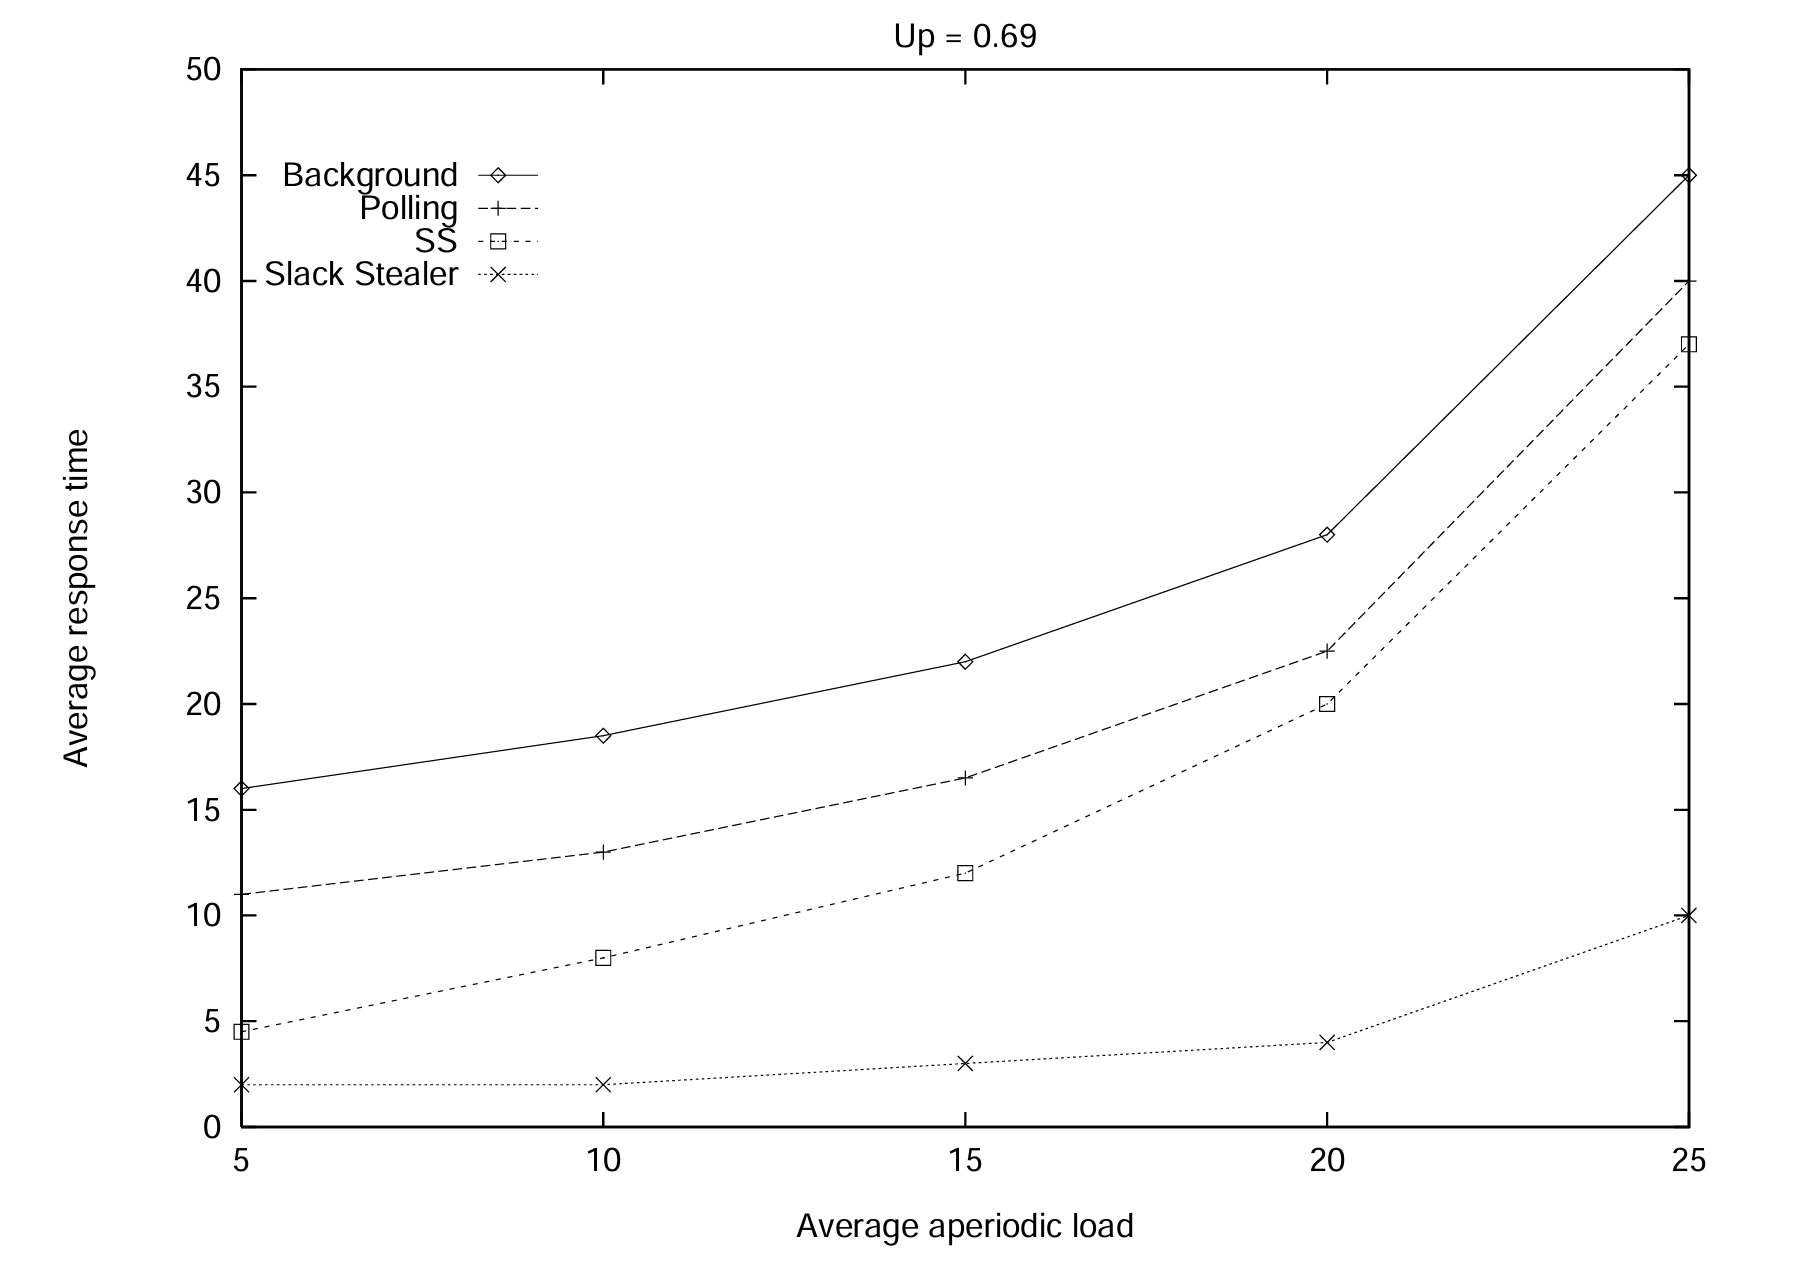
\includegraphics[width=0.7\textwidth]{pictures/performanceComparison.png}
    \caption{Performance dei server}
    \label{fig:performanceComparison}
\end{figure}
\begin{figure}[H]
    \centering
    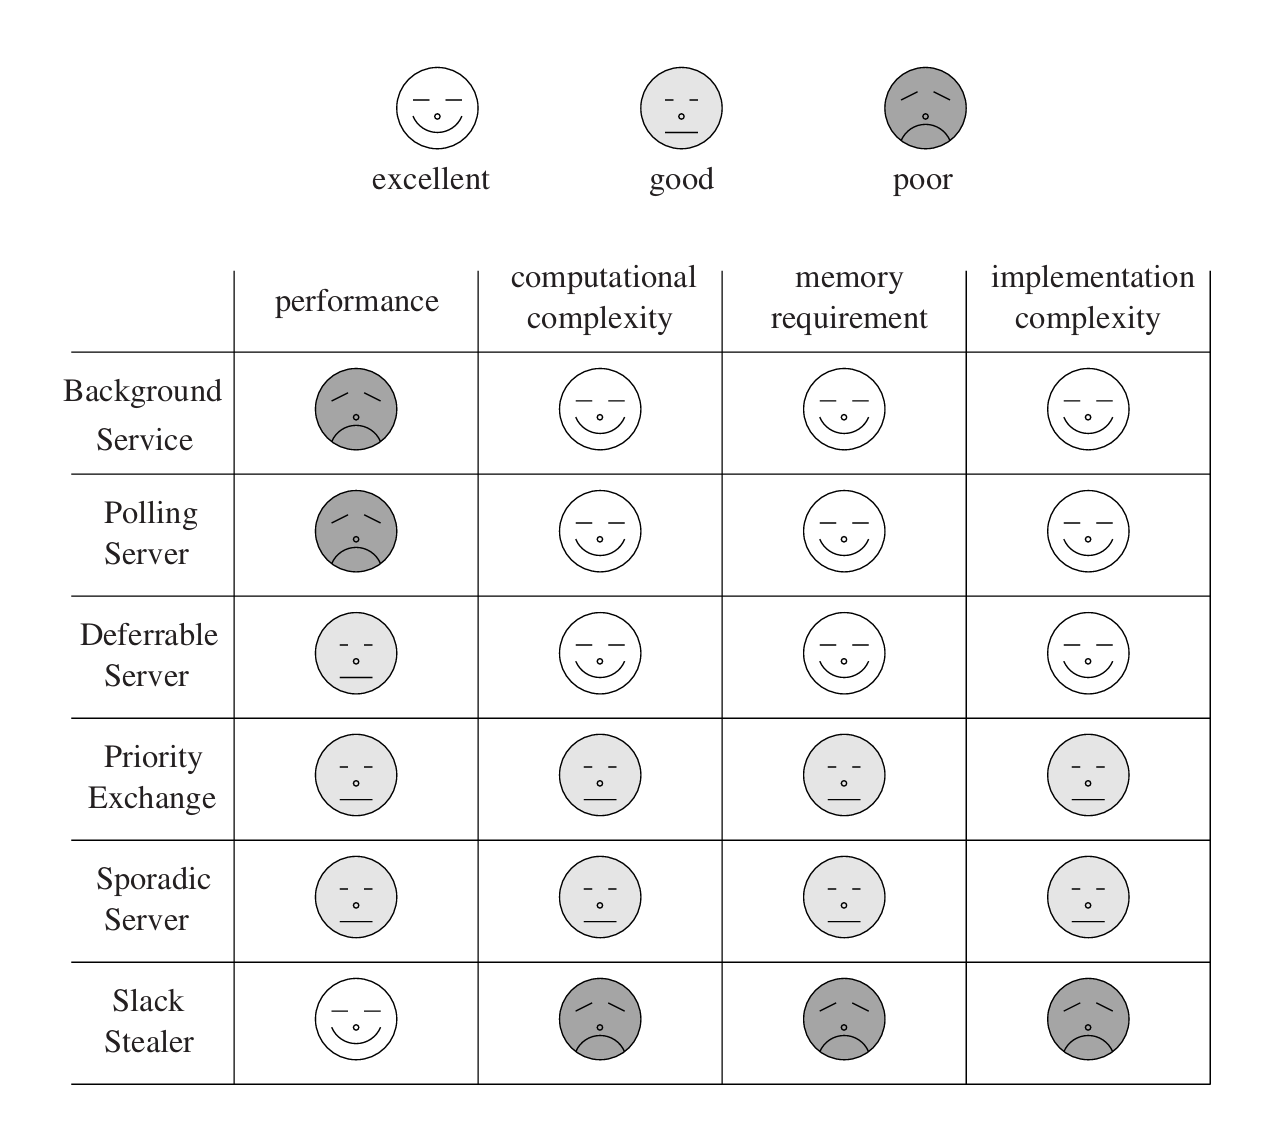
\includegraphics[width=0.7\textwidth]{pictures/comparisonServer.png}
    \caption{Confronto overall dei server}
    \label{fig:comparisonServer}
\end{figure}
\section{Server a priorità dinamica}
In questa sezione si discute il problema dello schedulare task soft aperiodici e task hard periodici in un sistema a priorità dinamica.
In particolare l'obbiettivo è ridurre il tempo di risposta medio delle richieste aperiodiche, senza degradare la schedulabilità di task hard periodici.
I task periodici vengono schedulati con EDF (dunque il fattore di utilizzo massimo del processore è 1).
L'aumentare del fattore di utilizzo massimo rispetto a RM (0.69) è vantaggioso perché ci permette di aumentare la dimensione massima dei server i.e. $U_s = 1- U_p$.
Per semplicità facciamo le seguenti assunzioni:
\begin{itemize}
\item Tutti i task periodici hanno deadline hard e la loro schedulabilità deve essere garantita off-line.
\item Tutti i task aperiodici non hanno deadline e devono essere schedulati il prima possibile, senza compromettere la schedulabilità dei task periodici.
\item La deadline dei task periodici è uguale al loro periodo.
\item Tutti i task periodici vengono attivati a tempo $t=0$.
\item Tutti i task aperiodici hanno tempo di computazione noto, ma tempo di arrivo arbitrario.
\end{itemize}
\subsection{Dynamic priority exchange server}
\label{sec:dynamicPriorityExchange}
Può essere visto come un'estensione del priority exchange server affrontato nella sezione \ref{sec:priorityExchange}.
L'idea principale è di lasciare che il se rver scambi il suo runtime con il runtime di task periodici di priorità più bassa (in EDF ciò significa deadline più lontana) nel caso non ci siano richieste aperiodiche in attesa.
In questo modo il runtime del server viene scambiato con il runtime di task periodici, ma mai sprecato perché verrà poi riscattato quando un task aperiodico arriva.
\subsubsection{Utilizzare lo spare time}
Nei sistemi hard real-time la garanzia viene effettuata sulla base del worst case scenario, ma quando non viene raggiunto il worst case vi è un tempo di esecuzione minore del WCET.
Usando un server DPE, il tempo che avanza può essere facilmente utilizzato per eseguire task aperiodici.
Questo viene fatto aggiungendo lo spare time dei task periodici alla capacità del server corrispondente.
Da notare che utilizzare lo spare time in questo modo non influisce sulla schedulabilità del sistema.
\subsection{Dynamic sporadic server}
\label{sec:dynamicSporadicServer}
Estensione di sporadic server, trattato nella sezione \ref{sec:sporadicServer}. A differenza di altri server la sua capacità non viene ricaricata a ogni periodo, ma solo quando viene completamente consumata.
La differenza con lo sporadic server classico è nella priorità del server. SS ha una priorità fissa e viene schedulato con RM, mentre DSS ha una priorità dinamica assegnata in base alla deadline adatta.
\subsection{Total bandwidth server}
\label{sec:totalBandwidthServer}
Osservando l'approccio del dynamic sporadic server è facilmente notabile che, quando il server ha un periodo lungo, l'esecuzione di task aperiodici può essere ritardata per un lungo periodo di tempo.
Una soluzione è assegnare una deadline più vicina a ogni task aperiodico, questo assegnamento deve essere fatto in maniera che l'utilizzo complessivo del processore non superi mai $U_s$.
Il nome viene dal fatto che quando una richiesta aperiodica entra nel sistema, l'intera bandwidth del server viene assegnata a essa, se possibile.
\subsection{Earliest deadline late server}
\label{sec:earliestDeadlineLateServer}
Versione dinamica dello slack stealer trattato nella sezione \ref{sec:slackStealing}.
Utilizziamo i tempi morti per schedulare i task aperiodici il prima possibile.
Quando non ci sono task aperiodici nel sistema (e nessun task periodico è attivo) il tempo che avanza viene utilizzato prima per i task periodici e poi per quelli aperiodici.
\subsection{Improved priority exchange server}
Nonostante sia ottimo, EDL ha troppo runtime overhead per essere considerato nella pratica.
La pesante computazione può essere evitata utilizzando il meccanismo di priority exchange.
I tempi morti di EDL possono essere pre calcolati off-line e il server può usarli per schedulare richieste aperiodiche (quando ci sono), o per eseguire task periodici.
Nel secondo caso il tempo morto può essere considerato come capacità del server per task aperiodici al livello di priorità del task periodico.
\subsection{Constant bandwith server}
\label{sec:constantBandwidthServer}
Come DSS garantisce che, se $U_s$ è la frazione di tempo di CPU utilizzata dal server, il contributo totale del server al fattore utilizzo è minore di $U_s$ anche in caso di overload.
Con CBS si ottengono performance molto migliori rispetto a DSS, confrontabili con quelle ottenibili con TBS.
Quando un nuovo task entra nel sistema gli viene assegnata una deadline adatta e viene inserito nella ready queue di EDF.
Se il task tenta di eseguire più del previsto la sua deadline viene spostata in avanti (ovvero la priorità diminuisce) per ridurre l'interferenza con gli altri task.



\end{document}
